%% Copernicus Publications Manuscript Preparation Template for LaTeX Submissions
%% ---------------------------------
%% This template should be used for copernicus.cls
%% The class file and some style files are bundled in the Copernicus Latex Package which can be downloaded from the different journal webpages.
%% For further assistance please contact the Copernicus Publications at: publications@copernicus.org
%% http://publications.copernicus.org


%% Please use the following documentclass and Journal Abbreviations for Discussion Papers and Final Revised Papers.


%% 2-Column Papers and Discussion Papers
\documentclass[gmd, manuscript]{copernicus}



%% Journal Abbreviations (Please use the same for Discussion Papers and Final Revised Papers)

% Atmospheric Chemistry and Physics (acp)
% Advances in Geosciences (adgeo)
% Advances in Statistical Climatology, Meteorology and Oceanography (ascmo)
% Annales Geophysicae (angeo)
% ASTRA Proceedings (ap)
% Atmospheric Measurement Techniques (amt)
% Advances in Radio Science (ars)
% Advances in Science and Research (asr)
% Biogeosciences (bg)
% Climate of the Past (cp)
% Drinking Water Engineering and Science (dwes)
% Earth System Dynamics (esd)
% Earth Surface Dynamics (esurf)
% Earth System Science Data (essd)
% Fossil Record (fr)
% Geographica Helvetica (gh)
% Geoscientific Instrumentation, Methods and Data Systems (gi)
% Geoscientific Model Development (gmd)
% Geothermal Energy Science (gtes)
% Hydrology and Earth System Sciences (hess)
% History of Geo- and Space Sciences (hgss)
% Journal of Sensors and Sensor Systems (jsss)
% Mechanical Sciences (ms)
% Natural Hazards and Earth System Sciences (nhess)
% Nonlinear Processes in Geophysics (npg)
% Ocean Science (os)
% Primate Biology (pb)
% Scientific Drilling (sd)
% SOIL (soil)
% Solid Earth (se)
% The Cryosphere (tc)
% Web Ecology (we)



%% \usepackage commands included in the copernicus.cls:
%\usepackage[german, english]{babel}
%\usepackage{tabularx}
%\usepackage{cancel}
%\usepackage{multirow}
%\usepackage{supertabular}
%\usepackage{algorithmic}
%\usepackage{algorithm}
%\usepackage{float}
%\usepackage{subfig}
%\usepackage{rotating}

\usepackage{amsmath}
\usepackage{lineno}	% Dominik linenumbers
\usepackage{rotating}	% Dominik rotate table

\usepackage{marginnote} %Dominik for commments during drafting
\setlength{\marginparwidth}{35mm}


\begin{document}

%\linenumbers

\title{OMEN-SED 1.0: A new, numerically efficient sediment module for the coupling to Earth System Models}


% \Author[affil]{given_name}{surname}
\Author[1]{Dominik}{H\"ulse}
\Author[1, 2]{Sandra}{Arndt}
\Author[3]{Stuart}{Daines}
\Author[1, 4]{Andy}{Ridgwell}
\Author[2]{Pierre}{Regnier}

\affil[1]{School of Geographical Sciences, University of Bristol, Clifton, Bristol BS8 1SS, UK}
\affil[2]{Department of Earth and Environmental Sciences, Universit\'e Libre de Bruxelles, Brussels, Belgium}
\affil[3]{Earth System Science, University of Exeter, North Park Road, Exeter EX4 4QE, UK}
\affil[4]{Department of Earth Sciences, University of California, Riverside, CA 92521, USA}

%% The [] brackets identify the author with the corresponding affiliation. 1, 2, 3, etc. should be inserted.



\runningtitle{OMEN-SED 1.0 - a sediment model for Earth System Models}

\runningauthor{H\"ulse et al.}

\correspondence{Dominik H\"ulse (Dominik.Huelse@bristol.ac.uk)}



\received{}
\pubdiscuss{} %% only important for two-stage journals
\revised{}
\accepted{}
\published{}

%% These dates will be inserted by Copernicus Publications during the typesetting process.


\firstpage{1}

\maketitle



\begin{abstract}
Here we describe the first version of the Organic Matter ENabled SEDiment model (OMEN-SED 1.0).
\end{abstract}



\introduction  %% \introduction[modified heading if necessary]
%>>>
\marginnote{\textbf{DH}: How to include comments.}[-1cm]%<<<
%\textbf{Role of marine sediments for climate and global biogeochemical cycles:}\\
Marine surface sediments are key components in the Earth system. They host the largest carbon reservoir within the surficial Earth system, provide the only long term sink for atmospheric \chem{CO_2}, 
recycle nutrients and represent the most important geochemical archive used for deciphering past changes in biogeochemical cycles and climate. 
Physical and chemical processes in sediments (i.e. diagenetic processes) depend on the water column and vice versa: Diagenesis is mainly donor controlled, as it is fuelled by the external supply of solid material 
(e.g. organic matter, calcium carbonate, opal) from the water column and is affected by overlying bottom water concentrations of solutes. 
At the same time, diagenesis in the sediments transforms the deposited material and returns some of the resulting products (e.g. nutrients, DIC) to the water column. 
This so-called benthic-pelagic coupling is essential for understanding global biogeochemical cycles and climate \citep[e.g.][]{archer_effect_1994, soetaert_coupling_2000, archer_what_2000, mackenzie_sediments_2005}. 

Biological primary production of organic matter (OM, \chem{CH_2O} in equation \ref{eq:photosynthesis}) and the reverse process of degradation can be written in a greatly simplified reaction as:
\begin{reaction}
\chem{CO_2}+\chem{H_2O} \rightleftharpoons \chem{CH_2O} + \chem{O_2}.\label{eq:photosynthesis}
\end{reaction}
On geological timescales production of OM is generally greater than degradation which results in some organic matter being buried in marine sediments and oxygen accumulating in the atmosphere. 
Thus burial of OM leads to net oxygen input to, and \chem{CO_2} removal from the atmosphere \citep{berner_phanerozoic_2004}. 
On shorter timescales, the upper few meters of the sediments (i.e. early diagenesis) are specifically important as it is decided here if a substance is recycled to the water column or buried for a longer period of time in the 
deeper sediments \citep{hensen_benthic_2006}. 
Most biogeochemical cycles and reactions in this part of marine sediments can be related either directly or indirectly to the degradation of organic matter \citep[e.g][]{boudreau_reactive_1991, arndt_quantifying_2013}. 
Organic matter degradation releases metabolic \chem{CO_2} to the pore water, causing it to have a lower pH and provoking the dissolution of \chem{CaCO_3} \citep{emerson_carbon_1981}.
Oxygen and nitrate for instance, the most powerful electron acceptors, are consumed in the course of the degradation of organic matter, resulting in the release of ammonium and phosphate to the pore water. 
As such, changes in the degradation rate of OM can profoundly affect the oxygen and nutrient inventory of the ocean and thus primary productivity \citep{van_cappellen_benthic_1994, lenton_redfield_2000}. 
%From Soetart-review: As such, marine sediments can affect the nutrient inventory of the ocean, hence, primary productivity \citep{van_cappellen_benthic_1994}. 

% DH: more facts on sediments
%Furthermore, the sedimenst form an important sink for organic phosphorus and nitrogen. 
%Furthermore, burial of OM represents an important connection between carbon stored in more climate-relevant reservoirs like oceans, atmosphere, 
%and surficial sediments and carbon that is sequestered for much longer, geological timescales in sedimentary rock or coal \citep{mackenzie_sediments_2005, burdige_preservation_2007}. 

%\textcolor{red}{TODO:} Something on: Role of marine sediments for another time period , e.g. glacial/interglacial atmospheric p\chem{CO_2} cycles
Nutrient recycling from the sediments has been invoked by modelling and data studies to explain the occurance of extreme events in Earth history, for instance Oceanic Anoxic Events (OAEs) 
\citep[e.g.][]{mort_phosphorus_2007, tsandev_modeling_2009}. OAEs represent severe disturbances of the global carbon, oxygen and nutrient cycles of the ocean and are usually characterized 
by widespread bottom water anoxia and photic zone euxinia \citep{jenkyns_geochemistry_2010}. 
One way to explain the genesis and persistence of OAEs is increased oxygen demand due to enhanced primary productivity (PP). Increased nutrient inputs to fuel PP may have come from marine sediments as the 
burial efficiency of phosphorus declines when bottom waters become anoxic \citep{ingall_evidence_1994, van_cappellen_benthic_1994}. 
The recovery from OAE like conditions is thought to involve the permanent removal of excess \chem{CO_2} from the atmosphere and ocean by burying carbon in the form of organic matter in marine sediments 
\citep[e.g.][]{arthur_geochemical_1988, jarvis_black_2011}, which is consistent with the geological record of widespread black shale formation \citep{stein_accumulation_1986}. 
However, the overall amount, exact timing and the rate of organic matter burial remain a topic of an ongoing debate. 

% % Difference for oxic vs. anoxic sediments and impacts on atmospheric \chem{CO_2}. 
% % 
% % Give examples when and why important (also in Paleo-context).\\
% % 
% % - general dynamics: first e.g. \chem{CaCO_3} then nutrients and the OM! \\
% % - then more focus on paleo!\\
% % - glacial/interglacial atmospheric p\chem{CO_2} cycles\\ 
% % - maybe important for OMZ (see Kriest + Oschlies 2013)\\
% % - \\
% % - Carbon burial events 

%\textbf{Diagenetic Models:}\\
Therefore, globally quantifying the burial and degradation of organic matter in marine sediments and related biogeochemical dynamics is important for understanding climate and the cycling of many chemical elements on various timescales.
Such studies and quantifications are possible through the application of idealised mathematical representations of diagenesis, or so-called diagenetic models \citep[e.g.][]{berner_early_1980, boudreau1997diagenetic}.
The number of research questions that can be addressed with diagenetic models is infinite and a plethora of different approaches have been developed, mainly following two distinct directions \citep{arndt_quantifying_2013}. 
First, state-of-the art vertically resolved diagenetic models simulating all of the essential coupled redox and equilibrium reactions within marine sediments that control carbon burial and benthic recycling fluxes 
(e.g. BRNS, \citeauthor{aguilera_knowledge-based_2005}, \citeyear{aguilera_knowledge-based_2005}; 
MEDIA, \citeauthor{meysman_reactive_2003}, \citeyear{meysman_reactive_2003}; OMEXDIA, \citeauthor{soetaert_model_1996}, \citeyear{soetaert_model_1996}). These ``complete'', non-steady-state models generally use a so-called multi-G approach, 
thus dividing the bulk organic carbon pool into a number of compound classes that are characterised by different degradabilities $k_i$. Combining such a complex diagenetic model with an ocean biogeochemical model results in 
the most realistic benthic-pelagic coupling. However, the global applicability of this set-up is limited by the high computation cost of simulating all biogeochemical reactions in the sediments. 
The second group of models is less sophisticated and comprehensive than the ``complete'', non-steady-state diagenetic models and is used for the coupling to global Earth System Models 
(e.g. DCESS, \citeauthor{shaffer_presentation_2008}, \citeyear{shaffer_presentation_2008}; MEDUSA, \citeauthor{munhoven_glacialinterglacial_2007}, \citeyear{munhoven_glacialinterglacial_2007} or the model of \citet{heinze_global_1999}). 
In particular, these analytic models consider fewer biogeochemical reactions and assume that the sedimentary organic matter pool is composed 
of just a single or two discrete compound classes (1G or 2G approach respectively). % apply the so-called 1G approach, thus just representing a single organic matter pool which is degraded at a constant rate. 

% From Soetart-review:  this evidence of mutual interaction between the water column and the sediment
% beneath, most biogeochemical models for water column processes either neglect the sediments or apply
% a rather crude approximation for the benthic response.

%\textbf{How are sediments resolved in Earth System models:}\\
Even though there is potential to use more appropriate global sediment representations, in most current Earth System models sediment-water exchange of OM and chemical elements is either neglected or treated in a very 
simplistic way \citep{soetaert_coupling_2000, huelse_biopump_models_2017}. 
Most Earth system Models of Intermediate Complexity (EMICs) and also some of the higher resolution global carbon cycle models represent the sediment-water interface either as a reflective or a conservative/semi-reflective boundary 
\citep{huelse_biopump_models_2017}. 
Thus, all particulate material deposited on the seafloor is either instantaneously consumed (reflective boundary), or a fixed fraction is buried in the sediments (conservative/semi-reflective boundary). 
Both highly simplified approaches furthermore completely neglect the exchange of solute species through the sediment-water interface and, therefore, cannot resolve the complex benthic-pelagic coupling. 
However, due to their computational efficiency, both representations are often used in global biogeochemical models \citep[e.g.][]{najjar_impact_2007, ridgwell_marine_2007, goosse_description_2010}. 
A superior approach is the vertically integrated dynamic model, which represents the whole sediment column as a single box \citep{huelse_biopump_models_2017}. Here, OM deposited on the seafloor is added 
to the sediment box where it gets degraded and dissolved species diffuse through the sediment-water interface in accordance with these transformations. 
This approach thus ignores the vertical extent of the sediments and the temporary storage of dissolved species \citep{soetaert_coupling_2000}. Yet, it is computationally efficient and 
also allows differentiating between various fractions of organic matter. Most EMICs incorporate a vertically integrated dynamic model for particulate inorganic carbon only (i.e. mainly \chem{CaCO_3}) and just a few  
consider oxic-only sediment degradation of organic matter \citep{huelse_biopump_models_2017}. 
The most complex description of marine sediments in Earth System models are vertically resolved diagenetic models, solving the one-dimensional, fully coupled reaction-transport equation for multiple solid and dissolved species 
\citep[e.g.][]{berner_early_1980, boudreau1997diagenetic}. These models account for important transport processes (e.g. bioturbation, molecular diffusion and bioirrigation), resolve the coupled biogeochemical dynamics of dissolved species
and usually at least a part of the resulting characteristic redox-zonation of marine sediments \citep{soetaert_coupling_2000}. Examples of global carbon cycle models employing a vertically resolved diagenetic model are 
PISCES \citep{gehlen_reconciling_2006} and CLIMBER 3$\alpha$ \citep{ilyina_global_2013}, both using a version of \citet{heinze_global_1999}, however, just utilizing a 1G approach with a constant degradation rate constant. % and NORESM \citep{tjiputra_evaluation_2013} does not say anything if they just use the original oxic-only
None of the EMICs reviewed by \citet{huelse_biopump_models_2017} use such a sediment representation. 

% Sandra review: large scale of published model parameters illustrates the complex nature of organic matter dynamics! Very difficult to find global relationships to relate model parameters 
% to available environmental characteristics, such as water depth, deposition rate. 

%\textbf{Problem with that:} \\
Obviously, such simplifications can neither account for the observed vast structural complexity in natural organic matter and its resulting different degradation rates nor for the rapid decrease in 
OM degradability in the uppermost centimeters of the sediments \citep{arndt_quantifying_2013}. At least a 3G approach is necessary to accurately represent organic matter dynamics in this part of the sediments where most OM is 
degraded \citep[e.g.][]{soetaert_model_1996}. 
Furthermore, the spatial variability in benthic OM degradation kinetics is unknown at the global scale and reported rate constants can vary by almost 10 orders of magnitude \citep{arndt_quantifying_2013}.
Thus, a major challenge for diagenetic models is defining appropriate OM degradation rate constants which is either achieved 
through profile fitting for a specific site or, for global applications, the rate constants follow empirical relations with a related, readily available sediment characteristic such as water depth 
\citep{middelburg_empirical_1997}, sedimentation rate \citep{toth_organic_1977, tromp_global_1995} or OM flux \citep{boudreau1997diagenetic}. 
However, these relationships are mostly based on simple fitting exercises to limited data sets and show at the most a very weak trend and no statistically significant relationship \citep{arndt_quantifying_2013}. 
This creates considerable uncertainties when diagenetic models are coupled to global biogeochemical ocean models especially when applying the model for different geological timescales. % see: https://goldschmidtabstracts.info/2013/2270.pdf
Other model parameters implicitly accounting for processes not explicitly described are sedimentation and bioturbation rate and are generally related to water depth following \citet{middelburg_empirical_1997}.

% These parameters, in particular the OM degradation rate constants, are either derived through profile fitting for a specific site or, for global applications, follow empirical relations with a related, readily available sediment 
% characteristic such as water depth \citep{middelburg_empirical_1997}, sedimentation rate \citep{toth_organic_1977, tromp_global_1995} or OM flux \citep{boudreau1997diagenetic}. 
% Start with OM is composed of loads of different compound classes. 1G approach can't account for that. Need at least 3 different fractions. Then problem of defining degradation rate constants especially on a global scale. 
% Say how diverse the OM stuff is and how variable it is spatially. Need actually at least 3G approach...
% Vertically integrated and resolved sediment models of organic matter degradation need to be properly initialise (i.e. get realistic POC degradation rates, from \citep{soetaert_coupling_2000})
% How they usually quantify the rate of OM degradation (see Stolpovsky et al. 2015 or/and \citep{soetaert_coupling_2000, mackenzie_past_2004}.\\
% The spatial variability in e.g. benthic particulate organic carbon (POC) mineralization kinetics throughout the ocean is currently unknown. This creates considerable 
% uncertainties when diagenetic models are used to couple benthic and pelagic biogeochemical cycles in global models. see: https://goldschmidtabstracts.info/2013/2270.pdf \\[2ex]

%\textcolor{red}{TODO???:} \textbf{Alternative Model approaches} e.g. from coastal research\\[2ex]

%\textbf{Solution presented here:}\\
Here, we present the OrganicMatter ENabled SEDiment model (OMEN-SED 1.0), a new, one-dimensional, numerically efficient reactive transport model (RTM) 
that describes OM cycling as well as the associated dynamics of the most important terminal electron acceptors (TEAs, i.e. \chem{O_2}, \chem{NO_3}, \chem{SO_4}, \chem{CH_4}), 
related reduced substances (\chem{NH_4} \chem{H_2S}), macronutrients (\chem{PO_4}) and associated pore water quantities (\chem{ALK}, \chem{DIC}).  
%for the biogeochemical dynamics of organic matter,  related chemical elements (\chem{O}, \chem{N}, \chem{S}, \chem{P}) and associated pore water quantities (ALK, DIC) in deep-sea sediments. 
OMEN-SED's computational efficiency allows its coupling to Earth System Models of different complexities and therefore the investigation of coupled global biogeochemical dynamics over geological timescales. 
Here, the model is presented as a 2G-approach, however, a third, nondegradable OM pool can be added and furthermore OMEN-SED can easily be extended to a Multi-G approach. 
% (including one ``refractory'' OM pool, whose degradability is not relevant for the timescales considered)
%See Van Cappellen and Wang (1996): ``Metal cycling in surface sediments: Modeling the interplay or transport and reaction'' for some good basic info! 

\section{Model Description}
The following section provides a detailed description of the new model. Table \ref{table:reactions_processes} summarizes the biogeochemical reaction network and 
a glossary of parameters along with their respective units is provided in Tables \ref{table:sed-charac_transport-parameters} and \ref{table:reaction_parameters}.

\subsection {General Model Approach} \label{subsec:GeneralModelApproach}
The calculation of benthic return/uptake and burial fluxes is based on the vertically resolved conservation equation for solid and dissolved species in porous media is given by 
\citep[e.g.][]{berner_early_1980, boudreau1997diagenetic}:

\begin{equation} 
\frac{\partial \xi C_i}{\partial t}=-\frac{\partial F}{\partial z}+\xi \sum_j R_i^j \label{eq:Eq_generaldiagenetic}
\end{equation}

where $C_i$ is the concentration of the biogeochemical species $i$, $\xi$ equals the porosity $\phi$ for solute species and $(1-\phi)$ for solid species, hence represents the partitioning of species $i$ 
into the solute and dissolved phase. The term $z$ is the sediment depth, $t$ denotes the time, $F$ summarises the transport fluxes and $\sum_j R_i^j$ represents the sum of production/consumption rates $j$ 
that affect species $i$. The reaction network accounts for the most important primary and secondary redox reactions, equilibrium reactions, mineral dissolution and precipitation, as well as adsorption 
and desorption processes that affect the explicitly resolved chemical species. 

State-of-the-art reaction-transport models generally solve the ordinary differential equation (ODE) (eq. \ref{eq:Eq_generaldiagenetic}) numerically and thus allow to account for transient dynamics, 
depth-varying parameters or a high degree of coupling between different chemical species \citep[e.g.][]{soetaert_model_1996, aguilera_knowledge-based_2005}. 
Yet, numerical models are computational expensive, thus rendering their application in an Earth System Model framework prohibitive. An analytical solution of equation \eqref{eq:Eq_generaldiagenetic} 
provides an alternative and computational more efficient approach which enjoyed great popularity in the early days of diagenetic modelling and computer technology. % due to their low computational demands. 
However, early analytical models were often very problem-specific and only considered one or two coupled species \citep[e.g.][]{berner_idealized_1964}. \textcolor{red}{(e.g. Lehrman, Berner) ?? which other pub?}
Over the next decades, a number of more complex analytical models describing the coupled dynamics of OM degradation, TEAs and rediced substances in sediments were developed \citep[e.g.][]{billen1982modelling, goloway1982diagenetic, jahnke1982model}, 
before the boost in computing power enabled the development of fully-coupled, multi-species, numerical models \citep[e.g.][]{van1995metal, soetaert_model_1996}. 

\begin{figure}[htbp]
\begin{center}
	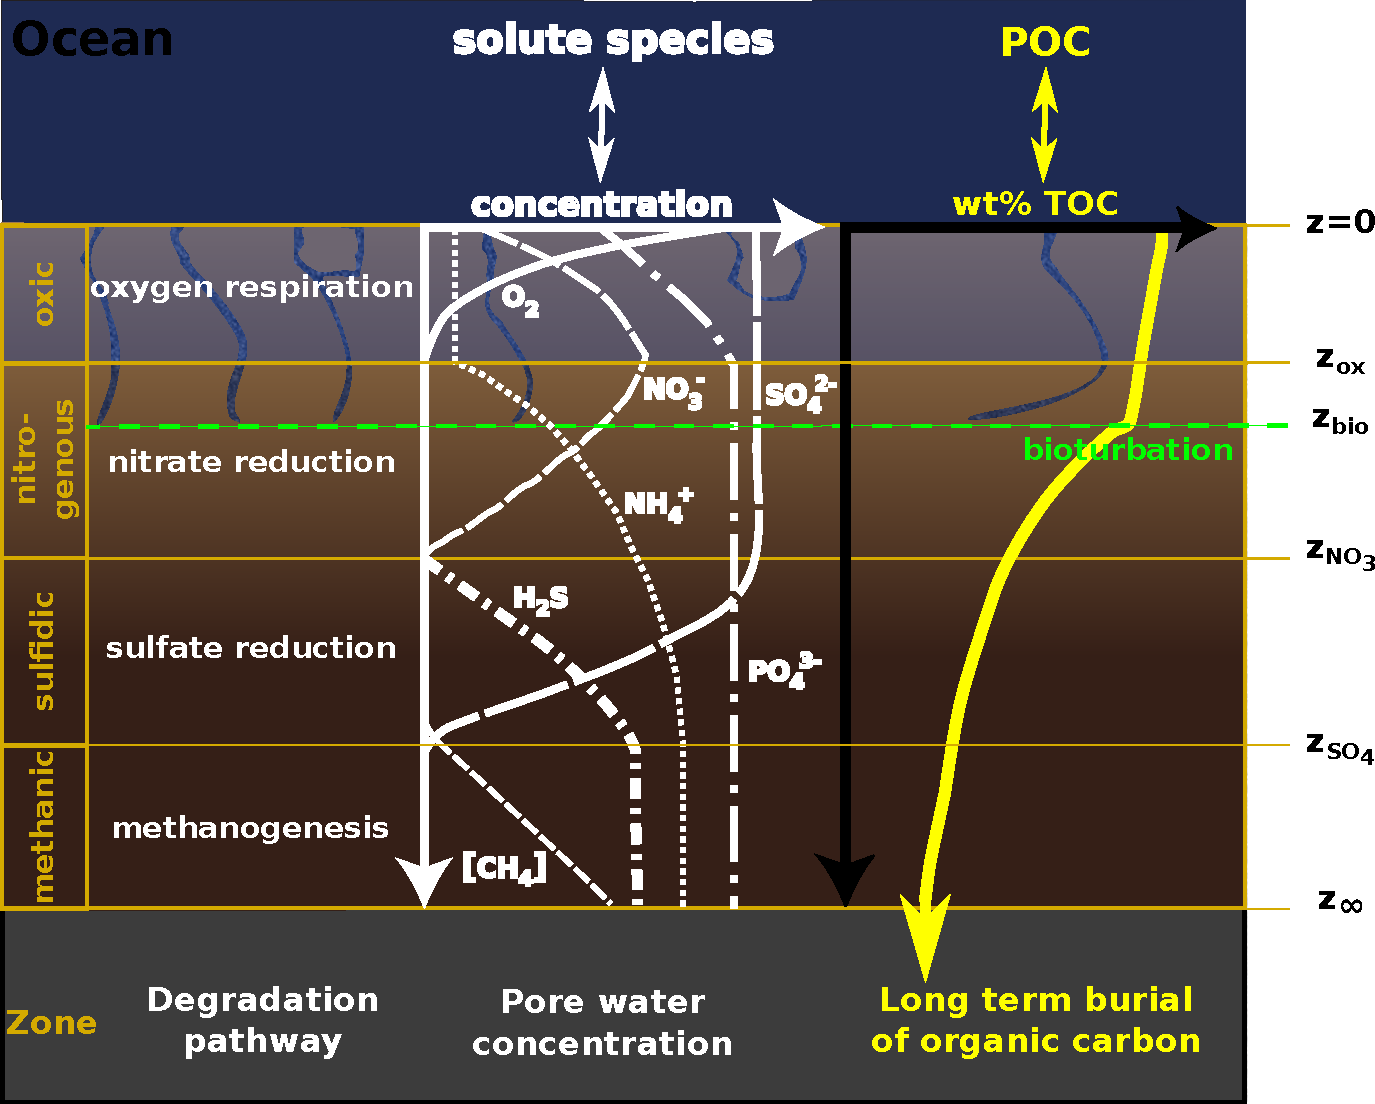
\includegraphics[width=0.8\textwidth]{figures/Sediment-model-with-profiles.pdf}
	\caption{Schematic of the different modelled species and layers in OMEN-SED (1.0). Here showing the case $z_{\mathrm{ox}} < z_{\mathrm{bio}} < z_{\chem{NO_3}} < z_{\chem{SO_4}}$.}
	\label{fig:Sediment_layers}
	\end{center}
\end{figure}

Finding an analytical solution to  Eq. (\ref{eq:Eq_generaldiagenetic}), especially when complex reaction networks are to be considered, is not straightforward and generally requires the assumption of steady state. 
In addition, the complexity of the reaction network can be reduced by dividing the sediment into distinct zones and accounting for the most pertinent biogeochemical processes 
within each zone, thus increasing the likelihood of finding an analytical solution to Eq. (\ref{eq:Eq_generaldiagenetic}) (see Eq. (\ref{eq:ODE_general_solution}) in section \ref{subsec:GBCM} for the general steady-state solution). 

Therefore, OMEN-SED assumes that benthic dynamics can be represented by a series of steady-states. 
Because the Earth system model relevant variability in boundary conditions and fluxes is generally longer than the characteristic timescales of the reaction-transport processes, the sediment can be described by a 
series of pseudo steady-states. In addition, it divides the sediment into a bioturbated and a non-bioturbated zone defined by the constant bioturbation depth $z_{\mathrm{bio}}$ (see Fig. \ref{fig:Sediment_layers}). 
Furthermore, it accounts for the dynamic redox zonation of marine sediments by dividing the sediment into: 2) an oxic zone delineated by the oxygen 
penetration depth $z_{\mathrm{ox}}$, 3) a denitrification zone situated between $z_{\mathrm{ox}}$ and the nitrate penetration depth $z_{\chem{NO_3}}$, 4) 
a sulfate reduction zone situated between $z_{\chem{NO_3}}$ and the sulfate penetration depth $z_{\chem{SO_4}}$ and 5) a methanogenic zone situated below $z_{\chem{SO_4}}$ (Fig. \ref{fig:Sediment_layers}). 
All penetration depths are dynamically calculated by the model. 
Each zone is characterised by a set of diagenetic equations that encapsulate the most pertinent reaction and transport processes in this zone (see section \ref{subsec:Transport} and \ref{subsec:ReactionNetwork} 
for more details). 

OMEN calculates and feeds back to the Earth System model the fraction of POC preserved in the sediments and the sediment-water interface fluxes of the dissolved species $C_i$ (in mol cm$^{-2}$ year$^{-1}$):
\begin{equation}
\mathrm{Flux\_SWI(C_i)} = \phi \left(D_i \frac{\partial C_i(z)}{\partial z}\bigg\rvert_0 - w \left[ C_i(0) - C_i(z_\infty) \right]\right)
\end{equation}
where $w$ is the deposition rate, $D_i$ is the diffusion coefficient and $C_i(0),\ C_i(z_\infty)$ the concentration of species $i$ at the SWI and at the lower sediment boundary. 

\subsection{Transport}\label{subsec:Transport}
The model accounts for both the advective, as well as the diffusive transport of dissolved and solid species, assuming that sediment compaction is negligible (i.e. $\frac{\partial \phi}{\partial z}=0$). 
The molecular diffusion of dissolved species is described via a species-specific apparent diffusion coefficient, $D_{\mathrm{mol},i}$. 
In addition, the activity of infaunal organisms in the bioturbated zone of the sediment ($z<z_{\mathrm{bio}}$) that causes random 
displacements of sediments and porewaters is simulated using a diffusive term (e.g. Boudreau,1986), with a constant bioturbation coefficient $D_{\mathrm{bio}}$ in the bioturbated zone. 
The pumping activity by burrow-dwelling animals and the resulting ventilation of tubes, the so-called bioirrigation, is encapsulated in a factor, $f_{ir}$ that enhances the molecular diffusion coefficient 
\citep[ hence, $D_{i,0}=D_{\mathrm{mol},i}\cdot f_{ir}$,][]{soetaert1996dynamic}. The flux divergence can thus be formulated as:
\begin{equation}
\frac{\partial F}{\partial z}=-\frac{\partial}{\partial z}\left( -\xi D_i \frac{\partial C_i}{\partial z} +\xi w C_i\right) \label{Eq_flux_divergence}
\end{equation}
where $D_i$ is the diffusion coefficient of species $i$ ($D_i=D_{i,0}+D_{\mathrm{bio}}=D_{\mathrm{mol},i}\cdot f_{ir}+D_{\mathrm{bio}}$ for dissolved species and $D_i=D_{\mathrm{bio}}$ for solid species) and $w$ is the 
deposition rate. 
The bioturbation coefficient $D_{\mathrm{bio}}$ is set to zero below $z_{\mathrm{bio}}$. In addition, infaunnal activity ceases ($D_{\mathrm{bio}}=0$) once bottom waters become anoxic ($\chem{O_2} < ???$ mol cm$^{-3}$ ). 
\textcolor{red}{check for good value + add if-query in code!!}

\subsection{Reaction Network}\label{subsec:ReactionNetwork}
Earth System models generally track the biogeochemical dynamics of organic and inorganic carbon, essential nutrients (nitrogen, phosphorus) and oxygen with the aim of investigating the evolution 
of the ocean's redox structure and carbonate system and its feedbacks on global climate. This general aim thus defines a minimum set of state variables and reaction processes that need to be resolved for an efficient 
representation of the benthic-pelagic coupling in Earth system models. A suitable sediment model must provide a robust quantification of organic (and inorganic) carbon burial fluxes, as well as 
the benthic return fluxes of growth-limiting nutrients, equilibrium invariant and reduced species, and oxygen uptake fluxes. 
As a consequence, the reaction network must account for the most important primary and secondary redox reactions, equilibrium reactions, 
mineral precipitation/dissolution and adsorption/desorption, resulting in a complex set of coupled reaction-transport equations. The following 
subsections provide a short discussion of the reaction processes included in the model and give an overview of the 
vertically resolved conservation equations and boundary conditions for solid and dissolved species in each layer. 
Table \ref{table:reactions_processes} provides a summary of the reactions and variables considered in the reaction network. Table \ref{table:Reaction_Network} summarises their reaction stoichiometry 
and Table \ref{table:ReactionOverview} provides an overview of their description in the model.

\begin{table}[tbp]
\caption{Reactions and variables implemented in the Reaction Network of OMEN-SED (1.0). The primary and secondary redox reactions are listed in the sequence they occur with increasing sediment depth.}
% title of Table
\centering
% used for centering table
\begin{tabular}{l l}
% centered columns (6 columns)
\hline\hline
%inserts double horizontal lines
 & Description\\
\hline
Primary redox reactions &  Degradation of organic matter via aerobic respiration, denitrification,\\
& sulfate reduction, methanogenesis (implicit)\\
Secondary redox reactions &  Oxidation of ammonium and sulfide by oxygen, anaerobic oxidation\\
& of methane by sulfate\\
Adsorption/Desorption & Ad-/Desorption of P on/from \chem{Fe(OH)_3}, \chem{NH_4} adsorption, \chem{PO_4} adsorption\\ %\textcolor{red}{Formation of Fe-bound P, reduction of Fe oxides (?correct here)},\\
Mineral precipitation & Formation of authigenic P \\
Variables & Organic matter, oxygen, nitrate, ammonium, sulfate, sulfide (hydrogen sulfide),\\
&  phosphate, Fe-bound P, DIC, ALK\\
\hline\hline
% inserts double horizontal lines
\end{tabular}
\label{table:reactions_processes}
% is used to refer this table in the text
\end{table}


\subsubsection{Organic matter or Particulate Organic Carbon (POC)}
In marine sediments, organic matter (OM) is degraded by heterotrophic activity coupled to the sequential utilisation of terminal electron acceptors, typically in the order of \chem{O_2}, \chem{NO_3^-}, \chem{Mn(VI)}, \chem{Fe(III)} and 
\chem{SO_4^{2-}} followed by methanogenesis and/or fermentation. Here, organic matter degradation is described via a multi-G model approach \citep[][and references therein]{arndt_quantifying_2013}, 
assuming that the bulk OM consists of a number of discrete compound classes $C_i$ characterised by specific degradation rate constants $k_i$. Such a multi-G approach allows for selective preservation of compound 
classes according to their reactivity, $k_i$ and, thus, accounts for the change in organic matter reactivity during burial. Each compound class is degraded according to first-order kinetics. 
The conservation equation for organic matter dynamics is thus given by:

\begin{equation}
 \frac{\partial C_i}{\partial t} = 0= D_{C_i} \frac{\partial^2C_i }{\partial z^2} - w\frac{\partial C_i }{\partial z} - k_i\cdot C_{i} \label{eq:ODE_OC}
\end{equation}
% where:
% \begin{align}
%  D_{C_i}&=D_{\mathrm{bio}} 	 &\text{if ($z\leq z_{\mathrm{bio}}$)}\\
%  D_{C_i}&=0            &\text{if ($z > z_{\mathrm{bio}}$)} 
% \end{align}
The analytical solution of Eq. \eqref{eq:ODE_OC} (see section \ref{subsec:module_Structure} for details) requires the definition of a set of boundary conditions (Table \ref{Tab:BC_OM}). 
The model assumes a known concentration/flux at the sediment-water interface and continuity across the bottom of the bioturbated zone, $z_{\mathrm{bio}}$.
\begin{table}[tbp]
\caption{Boundary conditions for organic matter. For the boundaries we define:  $z_{\mathrm{bio}}^- := \lim_{h\to0} (z_{\mathrm{bio}}-h)$ and $z_{\mathrm{bio}}^+ := \lim_{h\to0} (z_{\mathrm{bio}}+h)$.}
% title of Table
\centering
% used for centering table
\begin{tabular}{ |c| l| c l|}
\hline
\textbf{Boundary}& \textbf{Condition}& &\\
\hline
$z=0$& known concentration& 1)& $C_i(0)=C_{i0}$\\
$z=z_{\mathrm{bio}}$&continuity& 2)& $C_i(z_{\mathrm{bio}}^-)$=$C_i(z_{\mathrm{bio}}^+)$\\
               &&3)&$-D_{\mathrm{bio}}\cdot \frac{\partial C_i}{\partial z}|_{z_{\mathrm{bio}}^-}=0$\\
%Dom was               &&3) $D_{\mathrm{bio}}\cdot \frac{\partial C_i}{\partial z}|_{z_{\mathrm{bio}}^-}-w\cdot C_i(z_{\mathrm{bio}}^-)=-w\cdot C_i(z_{\mathrm{bio}}^+)$\\
\hline
\end{tabular}
\label{Tab:BC_OM}
% is used to refer this table in the text
\end{table}


\subsubsection{Oxygen}
In marine sediments, oxygen is consumed via aerobic degradation of organic matter and a number of secondary redox reactions. 
In the oxic layer ($z<z_{ox}$), the model explicitly accounts for the aerobic degradation of OM, which consumes oxygen with a fixed \chem{O_2:C} ratio (\chem{O_2C}, Tab. \ref{table:reaction_parameters}) 
and produces ammonium, which is partially nitrified to nitrate ($\gamma_\chem{NH_4}$).
%nitrification of parts of ammonium produced in the oxic layer of the sediment. 
%Oxygen serves as the most powerful terminal electron acceptor for the heterotrophic degradation of organic carbon. In addition, the oxidation of reduced species produced through microbial activity throughout the 
%sediment column further contributes to the consumption of oxygen. The model explicitly accounts for the consumption of oxygen by heterotrophic degradation and nitrification of ammonium in the oxic layer of the sediment. 
%The nitrification of 1 mol of ammonium in the oxic layer consumes 2 mol of oxygen. 
In addition, the oxygen consumption due to oxidation of reduced species (\chem{NH_4}, \chem{H_2S}) produced in the suboxic and anoxic layers of the sediment is implicitly taken into account 
through the flux boundary condition at the dynamic oxygen penetration depth $z_{\mathrm{ox}}$. This simplification can be justified as it has been shown that these secondary redox reactions mainly occur at the oxic/suboxic 
interface \citep{soetaert_model_1996}. The factor $\frac{1-\phi}{\phi}$ accounts for the volume conversion from the solid to the dissolved phase. 
%Oxygen is described in mol\,cm$^{-3}$ liquid and conversion from the solid phase of mineralized organic matter (expressed in mol\,cm$^{-3}$ bulk sediment) to consumption of dissolved oxygen (or later nutrients) introduce 
%a factor of $\frac{1-\phi}{\phi}$, where $\phi$ is the sediment porosity. 
Oxygen dynamics are thus described by:
\begin{align} 
 \frac{\partial \chem{O_2}}{\partial t} &= 0= D_{\chem{ \chem{O_2}}}\frac{\partial^2  \chem{O_2} }{\partial z^2} - w\frac{\partial  \chem{O_2}}{\partial z} - \frac{1-\phi}{\phi}\sum_i k_i \cdot [ \chem{O_2C} + 2 \gamma_{\chem{NH_4}} \chem{NC_i} ]\cdot C_{i}(z) \label{eq:ODE_O2_1}
\end{align}
% where:
% \begin{align}
%  D_{ \chem{O_2}}&=D_{ \chem{O_2}, 0}+D_{\mathrm{bio}}  &\text{if ($z\leq z_{\mathrm{bio}}$)}\\
%  D_{ \chem{O_2}}&=D_{ \chem{O_2}, 0}                &\text{if ($z > z_{\mathrm{bio}}$)} 
% \end{align}  
The analytical solution of Eq. \eqref{eq:ODE_O2_1} requires the definition of boundary conditions (Table \ref{Tab:BC_O2}). 
OMEN-SED (1.0) assumes a known bottom water concentration and the complete consumption of oxygen at the oxygen penetration depth (or zero flux if $z_{\mathrm{ox}}=z_\infty$). 
Equal oxygen concentration and diffusive flux above ($z_{\mathrm{bio}}^-$) and below ($z_{\mathrm{bio}}^+$) the bioturbation boundary is considered. 
In addition, the model accounts for reduced species produced by anaerobic mineralization diffusing into the oxic layer from below, 
assuming that respective fractions ($\gamma_{\chem{NH_4}}$ and $\gamma_{\chem{H_2S}}$) are re-oxidised at the oxic/suboxic interface. 

% was Sandra: In addition, it imposes a flux of reduce species through the bottom of the oxic zone that is calculated by integrating organic matter degradation rate and, thus, 
%assumes a complete oxidation of these species at the oxic/suboxic interface:   
\begin{table}[tbp]
\caption{Boundary conditions for oxygen. For the boundaries we define:  $z_{\mathrm{bio}}^- := \lim_{h\to0} (z_{\mathrm{bio}}-h)$ and $z_{\mathrm{bio}}^+ := \lim_{h\to0} (z_{\mathrm{bio}}+h)$.}
% title of Table
\centering
% used for centering table
\begin{tabular}{ |c| l| c l|}
\hline
\textbf{Boundary}& \textbf{Condition}& &\\
\hline
$z=0$& known concentration& 1)&$\chem{O_2}(0)=O_{20}$\\
$z=z_{\mathrm{bio}}$&continuity& 2)&$ \chem{O_2}(z_{\mathrm{bio}}^-)$=$ \chem{O_2}(z_{\mathrm{bio}}^+)$\\
               &&3)&$-\left(D_{ \chem{O_2},0}+D_{\mathrm{bio}}\right )\cdot \frac{\partial  \chem{O_2}}{\partial z}|_{z_{\mathrm{bio}}^-}=-D_{ \chem{O_2},0} \cdot \frac{\partial  \chem{O_2}}{\partial z}|_{z_{\mathrm{bio}}^+}$\\
%Dom was               &&3) $\left(D_{\mathrm{bio}}+D_{mol, \chem{O_2}}\right )\cdot \frac{\partial  \chem{O_2}}{\partial z}|_{z_{\mathrm{bio}}^-}-w\cdot  \chem{O_2}(z_{\mathrm{bio}}^-)=D_{mol, \chem{O_2}} \cdot \frac{\partial  \chem{O_2}}{\partial z}|_{z_{\mathrm{bio}}^+}-w\cdot  \chem{O_2}(z_{\mathrm{bio}}^+)$\\
$z=z_{\mathrm{ox}}$&  \chem{O_2} consumption & 4)&\textbf{IF} $ (\chem{O_2}(z_\infty)> 0 )$\\
& ($z_{\mathrm{ox}} = z_\infty$) &&\quad $\frac{\partial  \chem{O_2}}{\partial z}|_{z_{\mathrm{ox}}}=0$ \\
& & &\textbf{ELSE} \\
& ($z_{\mathrm{ox}} < z_\infty$) & &\quad $  \chem{O_2}(z_{\mathrm{ox}})=0$  \quad and \quad $-D_{ \chem{O_2}} \cdot \frac{\partial  \chem{O_2}}{\partial z}|_{z_{\mathrm{ox}}}=F_{red}(z_\mathrm{ox})$\\
%$z=z_{\mathrm{ox}}$& & 5) $-D_{ \chem{O_2}} \cdot \frac{\partial  \chem{O_2}}{\partial z}|_{z_{\mathrm{ox}}}=F_{red, z_{\mathrm{ox}}}$\\   
&with flux from below &&$\quad F_{red}(z_\mathrm{ox})=\frac{1-\phi}{\phi} \cdot \int_{z_{\mathrm{ox}}}^{\infty}  \sum_i \left( 2\gamma_{\chem{NH_4}} \chem{NC_i} + \gamma_{\chem{H_2S}} \chem{SO_4C} \right) k_i C_i\ dz$ \\
% was from Sandra &with:&$F_{red,z_{\mathrm{ox}}}=\beta \cdot \int_{z_{\mathrm{ox}}}^{\inf}  \sum_i k_i\cdot C_i  dz  + 2\cdot \gamma \cdot \int_{z_{\mathrm{ox}}}^{\inf}  \sum_i k_i\cdot C_i  -  $ \\
\hline    
\end{tabular}
\label{Tab:BC_O2}
% is used to refer this table in the text
\end{table}

\subsubsection{Nitrate and Ammonium}
%Nitrate and ammonium are described in $mol\ cm^{-3}$ liquid and a factor of $\frac{1-\phi}{\phi}$ is introduced to account for the conversion from mineralization rates to production of dissolved species. 
%To model nutrient dynamics the sediment is partitioned into two geochemical layers (oxic and suboxic)
To model nitrate and ammonium dynamics the sediment is partitioned into two geochemical layers (oxic and suboxic), where different equations describe the biogeochemical processes. 
Above the oxygen penetration depth organic matter mineralization produces ammonium, which is partly nitrified to nitrate (the fraction $\gamma_{\chem{NH_4}}$). 
In the suboxic zone ($z>z_{\mathrm{ox}}$), oxygen concentration is zero and nitrate serves as the electron acceptor to respire organic matter, thus nitrate is consumed by denitrification and ammonium is produced. Below the nitrate 
penetration depth $z_{\chem{NO_3}}$, ammonium is still produced via OM mineralization. The model assumes that adsorption of ammonium to sediment particles is fast compared with the characteristic transport time scales. 
Thus, a constant equilibrium adsorption coefficient $K_\chem{NH_4}$ is used to parameterize the loss of dissolved \chem{NH_4} to adsorped \chem{NH_4} \citep{wang_multicomponent_1996}.
Therefore the diagenetic equations for nitrate and ammonium are given by:
\begin{align}
\intertext{1. Layer ($z \leq z_{\mathrm{ox}}$)}
 \frac{\partial NO_3^I}{\partial t} &= 0 = D_{NO_3} \frac{\partial^2NO_3^I }{\partial z^2} - w\frac{\partial NO_3^I }{\partial z} + \gamma_{\chem{NH_4}} \frac{1-\phi}{\phi} \cdot \sum_i \chem{NC_i} \cdot k_i \cdot C_{i}(z)\label{eq:NO3_ODE1_L1}\\ %\qquad &\text{1. Layer ($z\leq z_{\mathrm{ox}}$)}\\
 \frac{\partial \chem{NH_4}^I}{\partial t} &= 0 = \frac{D_{\chem{NH_4}}}{1+K_\chem{NH_4}} \frac{\partial^2\chem{NH_4}^I }{\partial z^2} - w\frac{\partial \chem{NH_4}^I }{\partial z} + \frac{1-\gamma_{\chem{NH_4}}}{1+K_\chem{NH_4}}\cdot \frac{1-\phi}{\phi} \cdot \sum_i \chem{NC_i} \cdot k_i \cdot C_{i}(z)\label{eq:NH4_ODE1_L1}\\
 \intertext{2. Layer ($z_{\mathrm{ox}} < z \leq z_{\chem{NO_3}}$)} 
\frac{\partial NO_3^{II}}{\partial t} &= 0 = D_{NO_3} \frac{\partial^2NO_3^{II} }{\partial z^2} - w\frac{\partial NO_3^{II} }{\partial z} - \frac{1-\phi}{\phi} NO_3C \cdot \sum_i k_i \cdot C_{i}(z) \label{eq:NO3_ODE1_L2}\\
\frac{\partial \chem{NH_4}^{II}}{\partial t} &= 0 = \frac{D_{\chem{NH_4}}}{1+K_\chem{NH_4}} \frac{\partial^2\chem{NH_4}^{II} }{\partial z^2} - w\frac{\partial \chem{NH_4}^{II} }{\partial z} \label{eq:NH4_ODE1_L2}
 \intertext{3. Layer ($z_{\chem{NO_3}} < z \leq z_\infty$)} 
\frac{\partial \chem{NH_4}^{III}}{\partial t} &= 0 = \frac{D_{\chem{NH_4}}}{1+K_\chem{NH_4}} \frac{\partial^2\chem{NH_4}^{III} }{\partial z^2} - w\frac{\partial \chem{NH_4}^{III} }{\partial z} + \frac{1}{1+K_\chem{NH_4}}\cdot\frac{1-\phi}{\phi} \cdot \sum_i \chem{NC_i} \cdot k_i \cdot C_{i}(z)\label{eq:NH4_ODE1_L2}
\end{align}
% where
% \begin{align}
%  D_{i}&=D_{i, 0}+D_{\mathrm{bio}} &\text{if ($z\leq z_{\mathrm{bio}}$)}\\
%  D_{i}&=D_{i, 0}                &\text{if ($z > z_{\mathrm{bio}}$)} 
% \end{align} 
% and $i \in \{$NO$_3$, NH$_4\}$. 
The boundary conditions to solve Equations \ref{eq:NO3_ODE1_L1} - \ref{eq:NH4_ODE1_L2} are summarized in Table \ref{Tab:BC_NO3+NH4}. The model assumes known bottom water concentrations 
for both species, the complete consumption of nitrate at the nitrate penetration depth (or zero flux if $z_{\chem{NO_3}}=z_\infty$) and no change in ammonium flux at $z_\infty$. It considers equal concentrations and diffusive fluxes 
at $z_{\mathrm{bio}}$ and $z_{\mathrm{ox}}$.  In addition, the re-oxidation of upward-diffusing reduced ammonium is considered in the oxic-suboxic boundary condition for nitrate and ammonium. 

\begin{table}[tbp]
\caption{Boundary conditions for nitrate and ammonium. For the boundaries we define:  $z^-_{\_\_} := \lim_{h\to0} (z_{\_\_}-h)$ and $z^+_{\_\_} := \lim_{h\to0} (z_{\_\_}+h)$.}
% title of Table
\centering
% used for centering table
\begin{tabular}{ |c| c| c l|}
\hline
\textbf{Boundary}& \textbf{Condition}& &\\
\hline
$z=0$& known concentration& 1)& $NO_3(0)=NO_{30}$  \\
$z=z_{\mathrm{bio}}$&continuity& 2)& $NO_3(z_{\mathrm{bio}}^-)$=$NO_3(z_{\mathrm{bio}}^+)$\\
               && 3)& $-\left(D_{NO_3,0}+D_{\mathrm{bio}}\right )\cdot \frac{\partial NO_3}{\partial z}|_{z_{\mathrm{bio}}^-}=-D_{NO_3,0} \cdot \frac{\partial NO_3}{\partial z}|_{z_{\mathrm{bio}}^+}$\\
$z=z_{\mathrm{ox}}$& continuity& 4)& $NO_3(z_{\mathrm{ox}}^-)$=$NO_3(z_{\mathrm{ox}}^+)$\\
               && 5)& $-D_{NO_3} \cdot \frac{\partial NO_3}{\partial z}|_{z_{\mathrm{ox}}^-} + \gamma_{\chem{NH_4}}\cdot F_{\chem{NH_4}}(z_{\mathrm{ox}})=-D_{NO_3} \cdot \frac{\partial NO_3}{\partial z}|_{z_{\mathrm{ox}}^+}$\\
&where: & &$ F_{\chem{NH_4}}(z_{\mathrm{ox}})=\frac{1}{1+K_\chem{NH_4}}\cdot \frac{1-\phi}{\phi} \cdot \int_{z_{\chem{NO_3}}}^{\infty}  \sum_i k_i \cdot \chem{NC_i} \cdot C_i\ dz$ \\          
$z=z_{\chem{NO_3}}$& \chem{NO_3} consumption & 6) & \textbf{IF} $ (\chem{NO_3}(z_\infty)> 0 )$\\
& ($z_{\chem{NO_3}} = z_\infty$) & & \quad $\frac{\partial NO_3}{\partial z}|_{z_{\chem{NO_3}}}=0$\\
& & &\textbf{ELSE} \\
& ($z_{\chem{NO_3}} < z_\infty$) & &\quad $NO_3(z_{\chem{NO_3}})=0$ \\
% was from Sandra &with:&$F_{red,z_{\mathrm{ox}}}=\beta \cdot \int_{z_{\mathrm{ox}}}^{\inf}  \sum_i k_i\cdot C_i  dz  + 2\cdot \gamma \cdot \int_{z_{\mathrm{ox}}}^{\inf}  \sum_i k_i\cdot C_i  -  $ \\
\hline
$z=0$& known concentration& 1)& $\chem{NH_4}(0)= \chem{NH_{40}}$  \\
$z=z_{\mathrm{bio}}$&continuity& 2)& $\chem{NH_4}(z_{\mathrm{bio}}^-)$=$\chem{NH_4}(z_{\mathrm{bio}}^+)$\\
               && 3)& $-\frac{D_{\chem{NH_4},0}+D_{\mathrm{bio}}}{1+K_\chem{NH_4}}\cdot \frac{\partial \chem{NH_4}}{\partial z}|_{z_{\mathrm{bio}}^-}=-\frac{D_{\chem{NH_4},0}}{1+K_\chem{NH_4}} \cdot \frac{\partial \chem{NH_4}}{\partial z}|_{z_{\mathrm{bio}}^+}$\\
$z=z_{\mathrm{ox}}$& continuity& 4)& $\chem{NH_4}(z_{\mathrm{ox}}^-)$=$\chem{NH_4}(z_{\mathrm{ox}}^+)$\\
  & & 5)& $-\frac{D_{\chem{NH_4}}}{1+K_\chem{NH_4}} \cdot \frac{\partial \chem{NH_4}}{\partial z}|_{z_{\mathrm{ox}}^-} -\gamma_{\chem{NH_4}}\cdot F_{\chem{NH_4}}(z_{\mathrm{ox}})=-\frac{D_{\chem{NH_4}}}{1+K_\chem{NH_4}} \cdot \frac{\partial \chem{NH_4}}{\partial z}|_{z_{\mathrm{ox}}^+}$\\
&where: & & $F_{\chem{NH_4}}(z_{\mathrm{ox}})=\frac{1}{1+K_\chem{NH_4}}\cdot \frac{1-\phi}{\phi} \cdot \int_{z_{\chem{NO_3}}}^{\infty}  \sum_i k_i \cdot \chem{NC_i} \cdot C_i\ dz$ \\          
$z=z_{\chem{NO_3}}$&continuity& 6)& $\chem{NH_4}(z_{\chem{NO_3}}^-)$=$\chem{NH_4}(z_{\chem{NO_3}}^+)$\\
               & flux & 7)& $-\frac{D_{\chem{NH_4}}}{1+K_\chem{NH_4}}\cdot \frac{\partial \chem{NH_4}}{\partial z}|_{z_{\chem{NO_3}}^-}=-\frac{D_{\chem{NH_4}}}{1+K_\chem{NH_4}} \cdot \frac{\partial \chem{NH_4}}{\partial z}|_{z_{\chem{NO_3}}^+}$\\
$z=z_{\infty}$& zero \chem{NH_4} flux & 8)& $\frac{\partial \chem{NH_4}}{\partial z}|_{z_\infty}=0$\\
\hline    
\end{tabular}
\label{Tab:BC_NO3+NH4}
\end{table}
\subsubsection{Sulfate and Sulfide}
When nitrate is depleted, sulfate reduction is the pathway to mineralize organic matter, thus consuming sulfate (SO$_4$) and producing hydrogen sulfide (H$_2$S) until the sulfate penetration depth ($z_{\chem{\chem{SO_4}}}$). 
Sulfate and sulfide dynamics are thus described by:
\begin{align}
\intertext{1. Layer ($z \leq z_{\chem{NO_3}}$)}
 \frac{\partial \chem{SO_4}^I}{\partial t} &= 0 = D_{\chem{SO_4}} \frac{\partial^2\chem{SO_4}^I }{\partial z^2} - w\frac{\partial \chem{SO_4}^I }{\partial z} \label{eq:SO4_ODE1_L1}\\ %\qquad &\text{1. Layer ($z\leq z_{\mathrm{ox}}$)}\\
 \frac{\partial \chem{H_2S}^I}{\partial t} &= 0 = D_{\chem{H_2S}} \frac{\partial^2\chem{H_2S}^I }{\partial z^2} - w\frac{\partial \chem{H_2S}^I }{\partial z}\label{eq:H2S_ODE1_L1}\\
 \intertext{2. Layer ($z_{\chem{NO_3}} < z \leq z_{\chem{SO_4}}$)} 
\frac{\partial \chem{SO_4}^{II}}{\partial t} &= 0 = D_{\chem{SO_4}} \frac{\partial^2\chem{SO_4}^{II} }{\partial z^2} - w\frac{\partial \chem{SO_4}^{II} }{\partial z} - \frac{1-\phi}{\phi} \cdot \sum_i \chem{SO_4C} \cdot k_i \cdot C_{i}(z) \label{eq:SO4_ODE1_L2}\\
\frac{\partial \chem{H_2S}^{II}}{\partial t} &= 0 = D_{\chem{H_2S}} \frac{\partial^2\chem{H_2S}^{II} }{\partial z^2} - w\frac{\partial \chem{H_2S}^{II} }{\partial z} + \frac{1-\phi}{\phi} \cdot \sum_i \chem{SO_4C}  \cdot k_i \cdot C_{i}(z)\label{eq:H2S_ODE1_L2}
 \intertext{3. Layer ($z_{\chem{SO_4}} < z \leq z_{\infty}$)} 
\frac{\partial \chem{H_2S}^{III}}{\partial t} &= 0 = D_{\chem{H_2S}} \frac{\partial^2\chem{H_2S}^{III} }{\partial z^2} - w\frac{\partial \chem{H_2S}^{III} }{\partial z}\label{eq:H2S_ODE1_L3}
\end{align}
% where
% \begin{align}
%  D_{i}&=D_{i, 0}+D_{\mathrm{bio}} &\text{if ($z\leq z_{\mathrm{bio}}$)}\\
%  D_{i}&=D_{i, 0}                &\text{if ($z > z_{\mathrm{bio}}$)} 
% \end{align} 
% and $i \in \{$SO$_4$, H$_2$S$\}$. 
To solve equations \ref{eq:SO4_ODE1_L1} - \ref{eq:H2S_ODE1_L3} the model assumes known concentrations at the sediment-water interface and continuity 
across the bioturbation depth and the nitrate penetration depth (see Table \ref{Tab:BC_SO4+H2S}). 
The re-oxidation of reduced \chem{H_2S} to \chem{SO_4} is considered in the 
oxic-suboxic boundary condition for both species, here including the methanic zone, as \chem{H_2S} is also produced during anaerobic oxidation of methane (AOM). 
Furthermore, sulfate is used at $z_{\chem{SO_4}}$ to oxidize methane from below and thus producing \chem{H_2S}. 
In case $z_{\chem{SO_4}}<z_\infty$, sulfate concentration is zero at $z_{\chem{SO_4}}$ and its diffusive flux must equal the amount of methane produced below; or, in case $z_{\chem{SO_4}}=z_\infty$, 
a zero flux condition for sulfate is considered. At the lower boundary $z_\infty$ zero flux of \chem{H_2S} is considered. 
%Additionally H$_2$S is produced by AOM which is considered in the flux boundary condition at $z_{\chem{SO_4}}$. 
\textcolor{red}{correct??}\\

\begin{table}[tbp]
\caption{Boundary conditions for sulfate and sulfide. For the boundaries we define:  $z^-_{\_\_} := \lim_{h\to0} (z_{\_\_}-h)$ and $z^+_{\_\_} := \lim_{h\to0} (z_{\_\_}+h)$.}
% title of Table
\centering
% used for centering table
\begin{tabular}{ |c| c| c l|}
\hline
\textbf{Boundary}& \textbf{Condition}&&\\
\hline
$z=0$& known concentration& 1)& \chem{SO_4}(0)=\chem{SO_{40}}  \\
$z=z_{\mathrm{bio}}$&continuity& 2)& $\chem{SO_4}(z_{\mathrm{bio}}^-)$=$\chem{SO_4}(z_{\mathrm{bio}}^+)$\\
               & flux & 3)& $-\left(D_{\chem{SO_4},0}+D_{\mathrm{bio}}\right )\cdot \frac{\partial \chem{SO_4}}{\partial z}|_{z_{\mathrm{bio}}^-}=-D_{\chem{SO_4},0} \cdot \frac{\partial \chem{SO_4}}{\partial z}|_{z_{\mathrm{bio}}^+}$\\
$z=z_{\mathrm{ox}}$& continuity& 4)& $\chem{SO_4}(z_{\mathrm{ox}}^-)$=$\chem{SO_4}(z_{\mathrm{ox}}^+)$\\
               & flux & 5)& $-D_{\chem{SO_4}} \cdot \frac{\partial \chem{SO_4}}{\partial z}|_{z_{\mathrm{ox}}^-} + \gamma_{\chem{H_2S}}\cdot F_{\chem{H_2S}}(z_{\mathrm{ox}})=-D_{\chem{SO_4}} \cdot \frac{\partial \chem{SO_4}}{\partial z}|_{z_{\mathrm{ox}}^+}$\\
&where:& &$\quad F_{\chem{H_2S}}(z_{\mathrm{ox}})=\frac{1-\phi}{\phi} \cdot \left( \int_{z_{\chem{NO_3}}}^{\chem{SO_4}}  \sum_i \chem{SO_4C} \cdot k_i \cdot C_i\ dz + \gamma_\chem{CH_4}\cdot \int_{z_{\chem{SO_4}}}^{\infty}  \sum_i \chem{MC} \cdot k_i \cdot C_i\ dz \right)$\\          
$z=z_{\chem{NO_3}}$&continuity& 6)& $\chem{SO_4}(z_{\chem{NO_3}}^-)$=$\chem{SO_4}(z_{\chem{NO_3}}^+)$\\
               & flux & 7)& $-D_{\chem{SO_4}}\cdot \frac{\partial \chem{SO_4}}{\partial z}|_{z_{\chem{NO_3}}^-}=-D_{\chem{SO_4}} \cdot \frac{\partial \chem{SO_4}}{\partial z}|_{z_{\chem{NO_3}}^+}$\\
$z=z_{\chem{SO_4}}$& SO$_4$ consumption & 8)&  \textbf{IF} $ (\chem{SO_4}(z_\infty)> 0 )$\\
& ($z_{\chem{SO_4}} = z_\infty$) && \quad $\frac{\partial SO_4}{\partial z}|_{z_{\chem{SO_4}}}=0$\\
& & &\textbf{ELSE} \\
& ($z_{\chem{SO_4}} < z_\infty$) && \quad $\chem{SO_4}(z_{\chem{SO_4}})=0$ \quad and \quad $-D_{\chem{SO_4}} \cdot \frac{\partial \chem{SO_4}}{\partial z}|_{z_{\chem{SO_4}}}= \gamma_\chem{CH_4} \cdot F_{\chem{CH_4}}(z_{\chem{SO_4}})$\\%\quad \textcolor{red}{or/and (???)} \quad $\frac{\partial \chem{SO_4}}{\partial z}|_{z_{\chem{SO_4}}}= 0$\\   
&with flux from below:& &$ \quad F_{\chem{CH_4}}(z_{\chem{SO_4}})=\frac{1-\phi}{\phi} \cdot \int_{z_{\chem{SO_4}}}^{\infty}  \sum_i \chem{MC} \cdot k_i \cdot C_i\ dz$ \\
% was from Sandra &with:&$F_{red,z_{\mathrm{ox}}}=\beta \cdot \int_{z_{\mathrm{ox}}}^{\inf}  \sum_i k_i\cdot C_i  dz  + 2\cdot \gamma \cdot \int_{z_{\mathrm{ox}}}^{\inf}  \sum_i k_i\cdot C_i  -  $ \\
\hline
$z=0$& known concentration& 1)& $\chem{H_2S}(0)=\chem{H_2S}_{0}$  \\
$z=z_{\mathrm{bio}}$&continuity& 2)& $\chem{H_2S}(z_{\mathrm{bio}}^-)$=$\chem{H_2S}(z_{\mathrm{bio}}^+)$\\
               & flux & 3)& $-\left(D_{\chem{H_2S},0}+D_{\mathrm{bio}}\right )\cdot \frac{\partial \chem{H_2S}}{\partial z}|_{z_{\mathrm{bio}}^-}=-D_{\chem{H_2S},0} \cdot \frac{\partial \chem{H_2S}}{\partial z}|_{z_{\mathrm{bio}}^+}$\\
$z=z_{\mathrm{ox}}$& continuity& 4)& $\chem{H_2S}(z_{\mathrm{ox}}^-)$=$\chem{H_2S}(z_{\mathrm{ox}}^+)$\\
               & flux & 5)& $-D_{\chem{H_2S}} \cdot \frac{\partial \chem{H_2S}}{\partial z}|_{z_{\mathrm{ox}}^-} - \gamma_\chem{H_2S}  F_{\chem{H_2S}}(z_{\mathrm{ox}})=-D_{\chem{H_2S}} \cdot \frac{\partial \chem{H_2S}}{\partial z}|_{z_{\mathrm{ox}}^+}$\\
&where: & &$\quad F_{\chem{H_2S}}(z_{\mathrm{ox}})=\frac{1-\phi}{\phi} \cdot \left( \int_{z_{\chem{NO_3}}}^{\chem{SO_4}}  \sum_i \chem{SO_4C} \cdot k_i \cdot C_i\ dz + \gamma_\chem{CH_4}\cdot \int_{z_{\chem{SO_4}}}^{\infty}  \sum_i \chem{MC} \cdot k_i \cdot C_i\ dz \right)$\\            
$z=z_{\chem{NO_3}}$&continuity& 6)& $\chem{H_2S}(z_{\chem{NO_3}}^-)$=$\chem{H_2S}(z_{\chem{NO_3}}^+)$\\
               & flux & 7)& $-D_{\chem{H_2S}}\cdot \frac{\partial \chem{H_2S}}{\partial z}|_{z_{\chem{NO_3}}^-}=-D_{\chem{H_2S}} \cdot \frac{\partial \chem{H_2S}}{\partial z}|_{z_{\chem{NO_3}}^+}$\\
$z=z_{\chem{SO_4}}$& continuity & 8)& $\chem{H_2S}(z_{\chem{SO_4}}^-)$=$\chem{H_2S}(z_{\chem{SO_4}}^+)$\\ %$\frac{\partial \chem{H_2S}}{\partial z}|_{z_{\chem{H_2S}}}=0$\\
               & flux (with AOM) & 9)&  $-D_{\chem{H_2S}}\cdot \frac{\partial \chem{H_2S}}{\partial z}|_{z_{\chem{SO_4}}^-} + \gamma_\chem{CH_4}\cdot F_{\chem{CH_4}}(z_{\chem{SO_4}})=-D_{\chem{H_2S}} \cdot \frac{\partial \chem{H_2S}}{\partial z}|_{z_{\chem{SO_4}}^+}$\\
&where: & &$\quad F_{\chem{CH_4}}(z_{\chem{SO_4}})=\frac{1-\phi}{\phi} \cdot \int_{z_{\chem{SO_4}}}^{\infty}  \sum_i \chem{MC} \cdot k_i \cdot C_i\ dz$ \\          
$z=z_{\infty}$& zero \chem{H_2S} flux & 10)& $\frac{\partial \chem{H_2S}}{\partial z}|_{z_\infty}=0$\\
\hline    
\end{tabular}
\label{Tab:BC_SO4+H2S}
%>>>
\marginnote{\textcolor{red}{\textbf{DH}: @Sandra: BC 5) Include $\int_{z_{\chem{\chem{SO_4}}}}^{\infty}$ here?}}[-13cm]%<<<
%>>>
\marginnote{\textcolor{red}{\textbf{DH}: @Sandra: think yes, because at 8) \chem{CH_4} from $\int_{z_{\chem{\chem{SO_4}}}}^{\infty}$ is oxidised to \chem{H_2S}; at 5) this \chem{H_2S} to \chem{SO_4}}}[-10.5cm]%<<<
\end{table}
% % % % Sulfate:\\
% % % % BC (5): Diffusive flux at $z_{\mathrm{ox}}$ is equal, considering the flux of reduced substances (H$_2$S) from below 
% % % % \textcolor{red}{(SD, matlab): flux discontinuity from H2S source; include methane region as AOM will produce sulfide as well(?)} \\
% % % % BC(9): matlab:Calculate SO4 consumption below zso4, by organic matter and indirectly via methane oxidation, \textcolor{red}{should it not be MC (methane to carbon ratio instead of SO4C}(???) \\
% % % % 
% % % % Sulfide:\\
% % % % BC (5): Match at zox, layer 1 - layer 2 (continuity, flux discontinuity from H2S source), flux of H2S to oxic interface (from all sources of H2S below), 
% % % % NB: include methane region as AOM will produce sulphide as well \textcolor{red}{should it be not the same as in SO4???}\\
% % % % BC (9): (flux with AOM production) flux of H2S produced by AOM interface (Source of H2S), \textcolor{red}{don't think the reaction conctants are correct in matlab!}


% \subsubsection{Ammonium}
% Processes considered\\
% general equation\\
% solution\\


\subsubsection{Phosphate}
\begin{figure}[htbp]
\begin{center}
	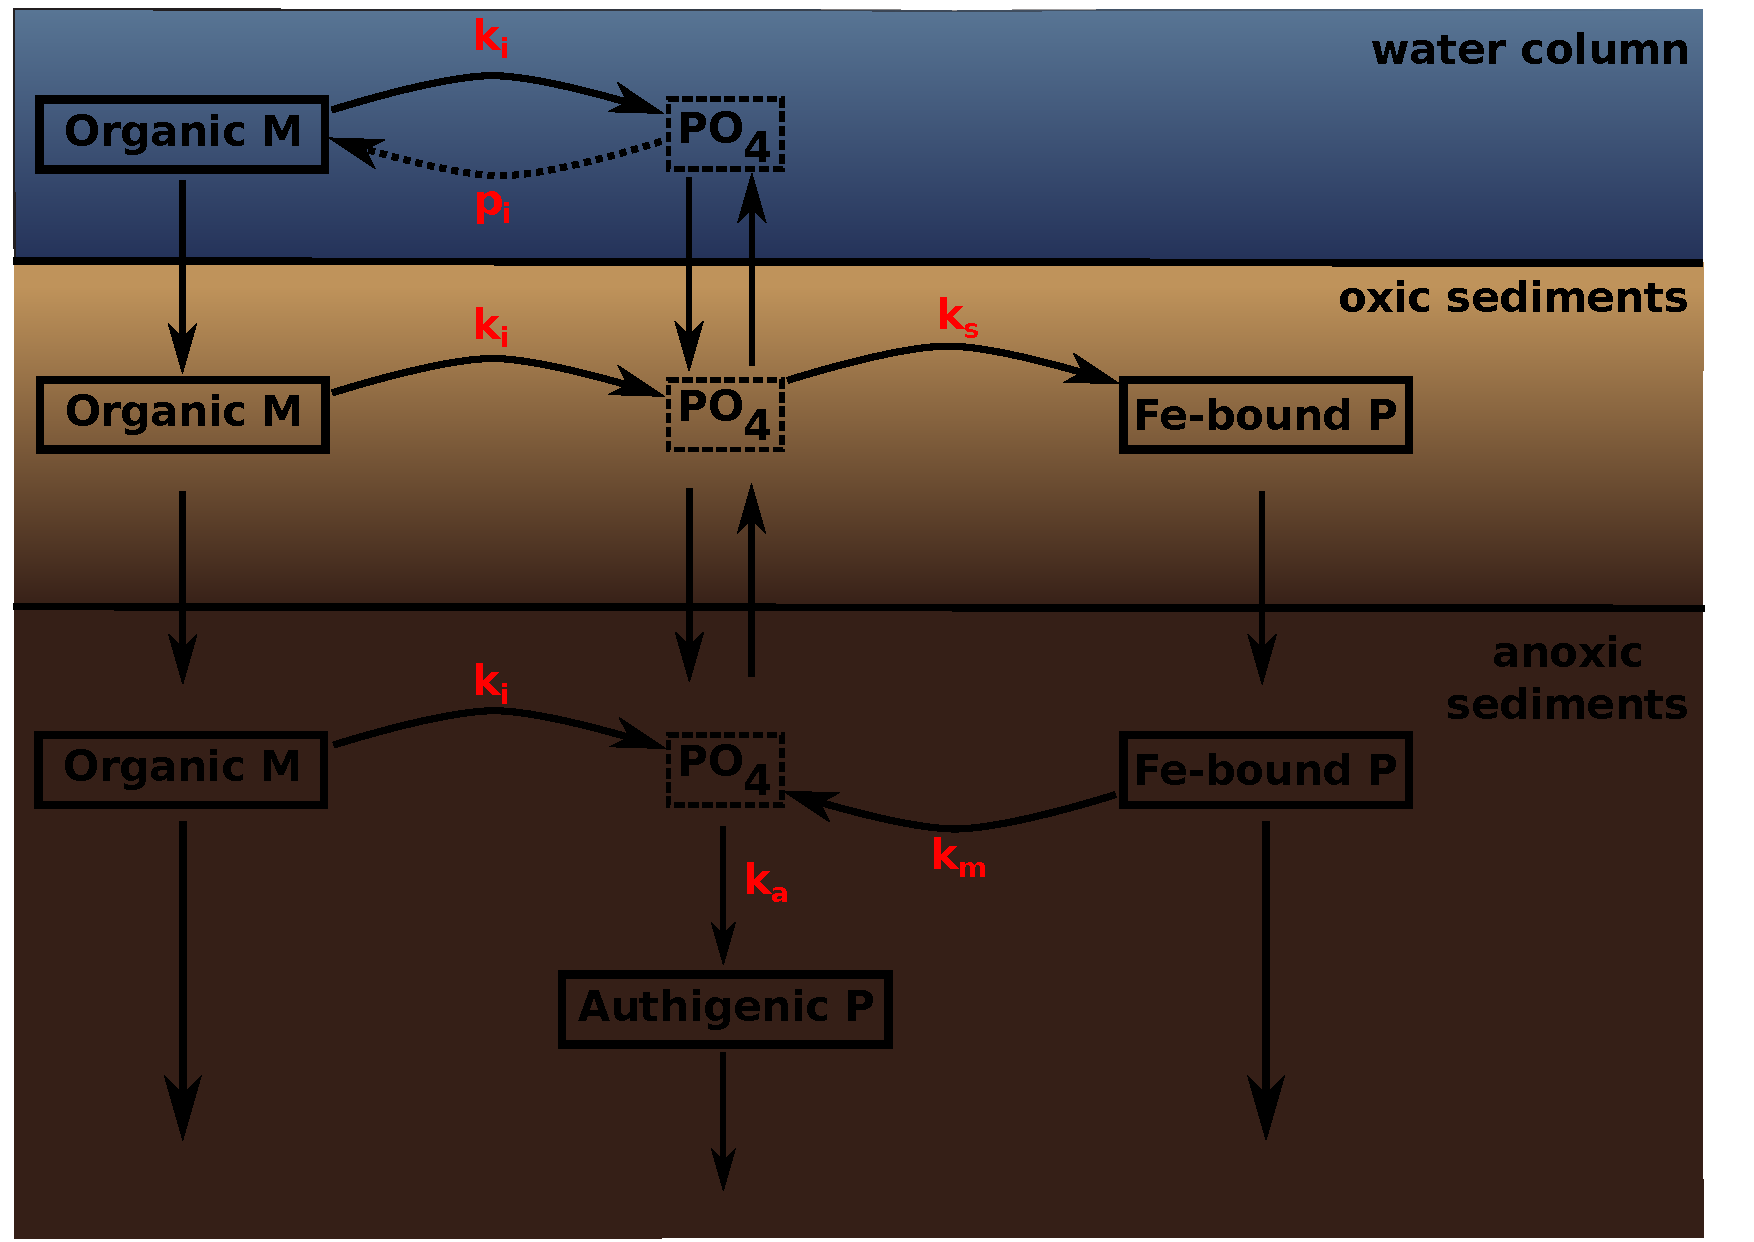
\includegraphics[width=0.8\textwidth]{figures/P-cycle.pdf}
	\caption{A schematic of the sedimentary P cycle in OMEN-SED (1.0). Red numbers represent kinetic rate constants for phosphorus dynamics (compare Table \ref{table:reaction_parameters}; p$_i$ represents uptake rate of PO$_4$ 
	via primary production in shallow environments). Adapted from \citet{caroline_p_slomp_key_1996}.}
	\label{fig:P-cycle}
	\end{center}
\end{figure}
To model phosphorus (P) dynamics in the sediments OMEN-SED takes into account the change with depth of phosphate (PO$_4$) and iron-bound P, thereby mainly following the description of \citet{caroline_p_slomp_key_1996} 
and \citet{gypens_simple_2008}. Throughout the sediment column organic matter is mineralized resulting in a release of phosphate to the pore water. In the oxic part of the sediment, this PO$_4$ either 
diffuses upward to the water column or is adsorped to Fe oxides forming Fe-bound P (or M) \citep{slomp1998role}. In the suboxic/anoxic zone, PO$_4$ is not only produced via organic matter degradation but is 
also released from the Fe-bound P pool due to the reduction of Fe oxides. Furthermore, phosphate concentrations can become high enough in this layer for authigenic mineral formation to occur \citep{cappellen_mathematical_1988}. 
This phosphorus bound in authigenic minerals represents a permanent sink for reactive phosphorus \citep{caroline_p_slomp_key_1996}. See Figure \ref{fig:P-cycle} for a schematic overview of the sedimentary P cycle. 
As for ammonium, the adsorption of P to the sediment matrix is treated as an equilibrium processes, parameterized with dimensionless adsorption coefficients for the oxic and anoxic zone 
\citep[$K_{\chem{PO_4}}^I$, $K_{\chem{PO_4}}^{II}$][]{slomp1998role}. Therefore the diagenetic equations for phosphate are written as:
\begin{align}
\intertext{1. Layer ($z \leq z_{\mathrm{ox}}$)}
 \frac{\partial \chem{PO_4}^I}{\partial t} &= \frac{D_{\chem{PO_4}}}{1+K_{\chem{PO_4}}^I} \frac{\partial^2\chem{PO_4}^I }{\partial z^2} - w\frac{\partial \chem{PO_4}^I }{\partial z} + \frac{1-\phi}{\phi}\frac{1}{1+K_{\chem{PO_4}}^I}\sum_i 
					\left( \chem{PC}_i \cdot k_i \cdot C_{i}(z) \right) \notag\\
					& - \frac{k_{s}}{1+K_{\chem{PO_4}}^I}(\chem{PO_4}^I-\chem{PO_4}^s)\label{eq:PO4_ODE_L1}\\  %&\text{1. Layer ($z\leq z_{\mathrm{ox}} \leq zbio$)}\label{eq:SO4_ODE1_Case1_sub1}\\
 \frac{\partial M^I}{\partial t} &= D_{M}\frac{\partial^2M^I }{\partial z^2} - w\frac{\partial M^I }{\partial z} + \frac{\phi}{1-\phi}k_{s}(\chem{PO_4}^I-\chem{PO_4}^s)\label{eq:M_ODE_L1}\\  
 \intertext{2. Layer ($z_{\mathrm{ox}} < z$)} 
 \frac{\partial M^{II}}{\partial t} & = D_{M}\frac{\partial^2M^{II} }{\partial z^2} - w\frac{\partial M^{II} }{\partial z} - k_{m}(M^{II} - M^\infty)\label{eq:M_ODE_L2}\\  
 \frac{\partial \chem{PO_4}^{II}}{\partial t} &= \frac{D_{\chem{PO_4}}}{1+K_{\chem{PO_4}}^{II}} \frac{\partial^2\chem{PO_4}^{II} }{\partial z^2} - w\frac{\partial \chem{PO_4}^{II} }{\partial z} + \frac{1-\phi}{\phi} \frac{1}{1+K_{\chem{PO_4}}^{II}}\sum_i 
					\left( \chem{PC}_i \cdot k_i \cdot C_{i}(z) \right) \notag\\
					& - \frac{k_{a}}{1+K_{\chem{PO_4}}^{II}}(\chem{PO_4}^{II}-\chem{PO_4}^a) + \frac{(1-\phi)}{\phi}\frac{k_{m}}{1+K_{\chem{PO_4}}^{II}}(M^{II}-M^\infty)\label{eq:PO4_ODE_L2}\\
\end{align}
% where
% \begin{align}
%  D_{\chem{PO_4}}&=D_{\chem{PO_4}, 0}+D_{\mathrm{bio}} &\text{ and }\quad D_{M}&= D_{\mathrm{bio}} &\text{if ($z\leq z_{\mathrm{bio}}$)}\\
%  D_{\chem{PO_4}}&=D_{\chem{PO_4}, 0} &\text{ and }\quad D_{M}&= 0 &\text{if ($z > z_{\mathrm{bio}}$)} 
% \end{align}
The boundary conditions to solve Equations \ref{eq:PO4_ODE_L1} - \ref{eq:PO4_ODE_L2} are summarized in Table \ref{Tab:BC_PO4+M}. 
The model assumes known bottom water concentrations and equal concentrations and diffusive fluxes at $z_{\mathrm{bio}}$ and $z_{\mathrm{ox}}$ for both species. 
Additionally it considers no change in phosphate flux and an assymptotic Fe-bound P concentration at $z_\infty$. \\

% TODO: \textcolor{red}{@ Sandra: SWI Flux for M does not exist, right???}

\begin{table}[tbp]
\caption{Boundary conditions for phosphate and Fe-bound P (M). For the boundaries we define:  $z^-_{\_\_} := \lim_{h\to0} (z_{\_\_}-h)$ and $z^+_{\_\_} := \lim_{h\to0} (z_{\_\_}+h)$.}
% title of Table
\centering
% used for centering table
\begin{tabular}{ |l| l| l|}
\hline
\textbf{Boundary}& \textbf{Condition}&\\
\hline
$z=0$& known concentration& 1) \chem{PO_4}(0)=\chem{PO_{40}}  \\
$z=z_{\mathrm{bio}}$&continuity& 2) $\chem{PO_4}(z_{\mathrm{bio}}^-)$=$\chem{PO_4}(z_{\mathrm{bio}}^+)$\\
               & flux & 3) $\left(D_{\chem{PO_4},0}+D_{\mathrm{bio}}\right )\cdot \frac{\partial \chem{PO_4}}{\partial z}|_{z_{\mathrm{bio}}^-}=D_{\chem{PO_4},0} \cdot \frac{\partial \chem{PO_4}}{\partial z}|_{z_{\mathrm{bio}}^+}$\\
$z=z_{\mathrm{ox}}$& continuity& 4) $\chem{PO_4}(z_{\mathrm{ox}}^-)$=$\chem{PO_4}(z_{\mathrm{ox}}^+)$\\
               & flux & 5) $-\frac{D_{\chem{PO_4}}}{1+K_{\chem{PO_4}}^I} \cdot \frac{\partial \chem{PO_4}}{\partial z}|_{z_{\mathrm{ox}}^-} =-\frac{D_{\chem{PO_4}}}{1+K_{\chem{PO_4}}^{II}} \cdot \frac{\partial \chem{PO_4}}{\partial z}|_{z_{\mathrm{ox}}^+}$\\
%&where:\textcolor{red}{$\int_{z_{\chem{SO_4}}}^{\infty}$ here?} & $\quad F_{\chem{H_2S}}(z_{\mathrm{ox}})=\frac{1-\phi}{\phi} \cdot \textcolor{red}{\gamma_{\chem{H_2S}}\cdot} \left( \int_{z_{\chem{NO_3}}}^{SO_4}  \sum_i SO_4C \cdot k_i \cdot C_i\ dz + \gamma_{CH_4}\cdot \int_{z_{\chem{SO_4}}}^{\infty}  \sum_i SO_4C \cdot k_i \cdot C_i\ dz \right)$\\          
$z=z_{\infty}$& flux & 10) $\frac{\partial \chem{PO_4}}{\partial z}|_{z_\infty}=0$\\
\hline
$z=0$& known concentration& 1) $M(0)=M_0$  \\
$z=z_{\mathrm{bio}}$&continuity& 2) $M(z_{\mathrm{bio}}^-)$=$M(z_{\mathrm{bio}}^+)$\\
  & flux & 3) $\frac{\partial M}{\partial z}|_{z_{\mathrm{bio}}^-}=\frac{\partial M}{\partial z}|_{z_{\mathrm{bio}}^+}$\\
$z=z_{\mathrm{ox}}$& continuity& 4) $M(z_{\mathrm{ox}}^-)$=$M(z_{\mathrm{ox}}^+)$\\
  & flux & 5) $\frac{\partial M}{\partial z}|_{z_{\mathrm{ox}}^-} =\frac{\partial M}{\partial z}|_{z_{\mathrm{ox}}^+}$\\
%&where:\textcolor{red}{$\int_{z_{\chem{SO_4}}}^{\infty}$ here?} & $\quad F_{\chem{H_2S}}(z_{\mathrm{ox}})=\frac{1-\phi}{\phi} \cdot \textcolor{red}{\gamma_{\chem{H_2S}}\cdot} \left( \int_{z_{\chem{NO_3}}}^{SO_4}  \sum_i SO_4C \cdot k_i \cdot C_i\ dz + \gamma_{CH_4}\cdot \int_{z_{\chem{SO_4}}}^{\infty}  \sum_i SO_4C \cdot k_i \cdot C_i\ dz \right)$\\          
$z=z_{\infty}$& assymptotic concentration & 10) $M(z_\infty)=M_\infty$\\
\hline    
\end{tabular}
\label{Tab:BC_PO4+M}
% is used to refer this table in the text
\end{table}
% \subsubsection{Sulfide}
% Processes considered\\
% general equation\\
% solution\\

\subsubsection{Dissolved Inorganic Carbon (DIC)}
Organic matter degradation produces dissolved inorganic carbon (DIC) with a stoichiometric DIC:C ratio of 1:2 in the methanic zone and 1:1 in the rest of the sediment column. 
DIC dynamics in OMEN-SED (1.0) are thus described by equations \ref{eq:DIC_ODE1_L1} and \ref{eq:DIC_ODE1_L1} and boundary conditions as summarized in Table \ref{Tab:BC_DIC}. 
The model assumes a known DIC concentration at the sediment-water interface, a zero flux condition at the lower boundary $z_\infty$ and continuity across the bioturbation and sulfate penetration depth. 
In addition, the anaerobic oxidation of methane at $z_{\chem{SO_4}}$ produces DIC (with 1:1 stoichiometry) which is accounted for through the flux boundary condition 
at $z_{\chem{SO_4}}$ (Table \ref{Tab:BC_DIC} eq. 5)

\begin{align}
\intertext{1. Layer ($z \leq z_{\chem{SO_4}}$)}
  \frac{\partial DIC^I}{\partial t} &= 0 = D_{DIC} \frac{\partial^2DIC^I }{\partial z^2} - w\frac{\partial DIC^I }{\partial z} + \frac{1-\phi}{\phi} \cdot \sum_i \chem{DICC^I} \cdot k_i \cdot C_{i}(z)\label{eq:DIC_ODE1_L1}\\ %\qquad &\text{1. Layer ($z\leq z_{\mathrm{ox}}$)}\\
 \intertext{2. Layer ($z_{\chem{SO_4}} < z \leq z_\infty$)} 
  \frac{\partial DIC^{II}}{\partial t} &= 0 = D_{DIC} \frac{\partial^2DIC^{II} }{\partial z^2} - w\frac{\partial DIC^{II} }{\partial z} + \frac{1-\phi}{\phi} \cdot \sum_i \chem{DICC^{II}} \cdot k_i \cdot C_{i}(z)\label{eq:DIC_ODE1_L2} %\qquad &\text{1. Layer ($z\leq z_{\mathrm{ox}}$)}\\
\end{align}

\begin{table}[tbp]
\caption{Boundary conditions for \chem{DIC}. For the boundaries we define:  $z^-_{\_\_} := \lim_{h\to0} (z_{\_\_}-h)$ and $z^+_{\_\_} := \lim_{h\to0} (z_{\_\_}+h)$.}
% title of Table
\centering
% used for centering table
\begin{tabular}{ |c| c| c l|}
\hline
\textbf{Boundary}& \textbf{Condition}&&\\
\hline
$z=0$& known concentration& 1)& $\chem{DIC}(0)=\chem{DIC}_{0}$  \\
$z=z_{\mathrm{bio}}$&continuity& 2)& $\chem{DIC}(z_{\mathrm{bio}}^-)$=$\chem{DIC}(z_{\mathrm{bio}}^+)$\\
               & flux & 3)& $-\left(D_{\chem{DIC},0}+D_{\mathrm{bio}}\right )\cdot \frac{\partial \chem{DIC}}{\partial z}|_{z_{\mathrm{bio}}^-}=-D_{\chem{DIC},0} \cdot \frac{\partial \chem{DIC}}{\partial z}|_{z_{\mathrm{bio}}^+}$\\
$z=z_{\chem{SO_4}}$& continuity & 4)& $\chem{DIC}(z_{\chem{SO_4}}^-)$=$\chem{DIC}(z_{\chem{SO_4}}^+)$\\ %$\frac{\partial \chem{DIC}}{\partial z}|_{z_{\chem{DIC}}}=0$\\
               & flux (with AOM) & 5)&  $-D_{\chem{DIC}}\cdot \frac{\partial \chem{DIC}}{\partial z}|_{z_{\chem{SO_4}}^-} + \gamma_\chem{CH_4}\cdot F_{\chem{CH_4}}(z_{\chem{SO_4}})=-D_{\chem{DIC}} \cdot \frac{\partial \chem{DIC}}{\partial z}|_{z_{\chem{SO_4}}^+}$\\
&where: & &$\quad F_{\chem{CH_4}}(z_{\chem{SO_4}})=\frac{1-\phi}{\phi} \cdot \int_{z_{\chem{SO_4}}}^{\infty}  \sum_i \chem{MC} \cdot k_i \cdot C_i\ dz$ \\          
$z=z_{\infty}$& zero \chem{DIC} flux & 6)& $\frac{\partial \chem{DIC}}{\partial z}|_{z_\infty}=0$\\
\hline
\end{tabular}
\label{Tab:BC_DIC}
\end{table}


\subsubsection{Alkalinity}
Organic matter degradation and secondary redox reactions exert a complex influence on alkalinity with opposite effects depending on the TEA involved \citep{wolf-gladrow_total_2007}. 
%The dynamics are further complicated by the influence of secondary redox reactions. 
To model alkalinity in OMEN-SED the sediment column is partitioned into four geochemical layers, where different equations describe the biogeochemical processes using variable stoichiometric coefficients 
(compare Tables \ref{table:reaction_parameters} and \ref{table:Reaction_Network}). 
Above $z_{\mathrm{ox}}$, aerobic OM mineralization decreases alkalinity according to $\chem{ALK}^\mathrm{OX}$ whereas nitrification increases alkalinity with stoichiometry $\chem{ALK}^\mathrm{NIT}$.
In the remaining three zones anaerobic OM mineralization increases alkalinity with variable stoichiometric coefficients (i.e. $\chem{ALK}^\mathrm{DEN}$, $\chem{ALK}^\mathrm{SUL}$, $\chem{ALK}^\mathrm{MET}$). 
Thus, the diagenetic equations for alkalinity are written as:
\begin{align}
 \intertext{1. Layer ($z \leq z_{\chem{ox}}$)} 
\frac{\partial \chem{ALK}^{I}}{\partial t} &= 0 = D_{\chem{ALK}} \frac{\partial^2\chem{ALK}^{I} }{\partial z^2} - w\frac{\partial \chem{ALK}^{I} }{\partial z} \notag\\
					  & + \frac{1-\phi}{\phi} \cdot \sum_i \left( \chem{ALK}^\mathrm{NIT} \cdot \frac{\gamma_{\chem{NH_4}}}{1+K_\chem{NH_4}} \chem{NC_i} + \chem{ALK}^\mathrm{OX}\right)\cdot k_i \cdot C_{i}(z) \label{eq:ALK_ODE1_L1}\\
 \intertext{2. Layer ($z_{\chem{ox}} < z \leq z_{\chem{NO_3}} $)} 
\frac{\partial \chem{ALK}^{II}}{\partial t} &= 0 = D_{\chem{ALK}} \frac{\partial^2\chem{ALK}^{II} }{\partial z^2} - w\frac{\partial \chem{ALK}^{II} }{\partial z} + \frac{1-\phi}{\phi} \cdot \sum_i \chem{ALK}^\mathrm{DEN}\cdot k_i \cdot C_{i}(z)\label{eq:ALK_ODE1_L2}
 \intertext{3. Layer ($z_{\chem{NO_3}} < z \leq z_{\chem{SO_4}} $)} 
\frac{\partial \chem{ALK}^{III}}{\partial t} &= 0 = D_{\chem{ALK}} \frac{\partial^2\chem{ALK}^{III} }{\partial z^2} - w\frac{\partial \chem{ALK}^{III} }{\partial z} + \frac{1-\phi}{\phi} \cdot \sum_i \chem{ALK}^\mathrm{SUL}\cdot k_i \cdot C_{i}(z)\label{eq:ALK_ODE1_L3}
 \intertext{4. Layer ($z_{\chem{SO_4}} < z \leq z_{\infty} $)} 
\frac{\partial \chem{ALK}^{IV}}{\partial t} &= 0 = D_{\chem{ALK}} \frac{\partial^2\chem{ALK}^{IV} }{\partial z^2} - w\frac{\partial \chem{ALK}^{IV} }{\partial z} + \frac{1-\phi}{\phi} \cdot \sum_i \chem{ALK}^\mathrm{MET}\cdot k_i \cdot C_{i}(z)\label{eq:ALK_ODE1_L4}
\end{align}
To solve equations \ref{eq:ALK_ODE1_L1} - \ref{eq:ALK_ODE1_L4} the model assumes a known concentration at the sediment-water interface and continuity 
across the bioturbation depth and the penetration depths of \chem{O_2}, \chem{NO_3} and \chem{SO_4} (see Table \ref{Tab:BC_ALK}). 
The decrease of alkalinity due to oxidation of reduced species produced in the suboxic and anoxic layers is implicitly taken into account 
through the flux boundary condition at $z_{\mathrm{ox}}$ (Table \ref{Tab:BC_ALK} eq. 5). 
Furthermore, the oxidation of methane by sulphate reduction increases alkalinity with stoichiometry $\chem{ALK}^\mathrm{AOM}$ which is accounted for through the flux boundary condition 
at $z_{\chem{SO_4}}$ (Table \ref{Tab:BC_ALK} eq. 9). At the lower boundary $z_\infty$ a zero flux condition is applied. 

\begin{table}[tbp]
\caption{Boundary conditions for alkalinity. For the boundaries we define:  $z^-_{\_\_} := \lim_{h\to0} (z_{\_\_}-h)$ and $z^+_{\_\_} := \lim_{h\to0} (z_{\_\_}+h)$.}
% title of Table
\centering
% used for centering table
\begin{tabular}{ |c| c| c l|}
\hline
\textbf{Boundary}& \textbf{Condition}&&\\
\hline
$z=0$& known concentration& 1)& $\chem{ALK}(0)=\chem{ALK}_{0}$  \\
$z=z_{\mathrm{bio}}$&continuity& 2)& $\chem{ALK}(z_{\mathrm{bio}}^-)$=$\chem{ALK}(z_{\mathrm{bio}}^+)$\\
               & flux & 3)& $-\left(D_{\chem{ALK},0}+D_{\mathrm{bio}}\right )\cdot \frac{\partial \chem{ALK}}{\partial z}|_{z_{\mathrm{bio}}^-}=-D_{\chem{ALK},0} \cdot \frac{\partial \chem{ALK}}{\partial z}|_{z_{\mathrm{bio}}^+}$\\
$z=z_{\mathrm{ox}}$& continuity& 4)& $\chem{ALK}(z_{\mathrm{ox}}^-)$=$\chem{ALK}(z_{\mathrm{ox}}^+)$\\
               & flux & 5)& $-D_{\chem{ALK}} \cdot \frac{\partial \chem{ALK}}{\partial z}|_{z_{\mathrm{ox}}^-} +  F_{\chem{ALK}}(z_{\mathrm{ox}})=-D_{\chem{ALK}} \cdot \frac{\partial \chem{ALK}}{\partial z}|_{z_{\mathrm{ox}}^+}$\\
&where: & &$\quad F_{\chem{ALK}}(z_{\mathrm{ox}})=\frac{1-\phi}{\phi} \cdot \left( \chem{ALK}^\chem{H_2S}\cdot \gamma_\chem{H_2S} \int_{z_{\chem{NO_3}}}^{\chem{SO_4}} \sum_i \chem{SO_4C} \cdot k_i \cdot C_i\ dz \right)$\\
& & &$\qquad \qquad \qquad \quad + \frac{1-\phi}{\phi} \cdot \left(\chem{ALK}^\chem{NIT} \frac{\gamma_\chem{NH_4}}{1+k_\chem{NH_4}}\int_{z_{\chem{NO_3}}}^{\infty}  \sum_i \chem{NC_i} \cdot k_i \cdot C_i\ dz \right)$\\            
$z=z_{\chem{NO_3}}$&continuity& 6)& $\chem{ALK}(z_{\chem{NO_3}}^-)$=$\chem{ALK}(z_{\chem{NO_3}}^+)$\\
               & flux & 7)& $-D_{\chem{ALK}}\cdot \frac{\partial \chem{ALK}}{\partial z}|_{z_{\chem{NO_3}}^-}=-D_{\chem{ALK}} \cdot \frac{\partial \chem{ALK}}{\partial z}|_{z_{\chem{NO_3}}^+}$\\
$z=z_{\chem{SO_4}}$& continuity & 8)& $\chem{ALK}(z_{\chem{SO_4}}^-)$=$\chem{ALK}(z_{\chem{SO_4}}^+)$\\ %$\frac{\partial \chem{ALK}}{\partial z}|_{z_{\chem{ALK}}}=0$\\
               & flux (with AOM) & 9)&  $-D_{\chem{ALK}}\cdot \frac{\partial \chem{ALK}}{\partial z}|_{z_{\chem{SO_4}}^-} + F_{\chem{ALK}}(z_{\chem{SO_4}})=-D_{\chem{ALK}} \cdot \frac{\partial \chem{ALK}}{\partial z}|_{z_{\chem{SO_4}}^+}$\\
&where: & &$\quad F_{\chem{ALK}}(z_{\chem{SO_4}})=\frac{1-\phi}{\phi} \cdot \left( \chem{ALK}^\chem{AOM}\gamma_\chem{CH_4}\cdot \int_{z_{\chem{SO_4}}}^{\infty}  \sum_i k_i \cdot C_i\ dz \right)$ \\          
$z=z_{\infty}$& zero \chem{ALK} flux & 10)& $\frac{\partial \chem{ALK}}{\partial z}|_{z_\infty}=0$\\
\hline    
\end{tabular}
\label{Tab:BC_ALK}
\end{table}

\subsection{Model Parameters}
This section describes the parameters used in OMEN-SED (1.0) to describe sediment transport and biogeochemical reactions related to the burial and mineralization of organic matter under a wide range of environmental conditions. 
Table \ref{table:sed-charac_transport-parameters} states the parameters for sediment characteristics and Table \ref{table:reaction_parameters} summarizes the stoichiometric factors and 
secondary reaction parameters used in the model.

\subsubsection{Transport Parameters}
Advection is the bulk flow of sediments and can be directly related to the accumulation of new material on the seafloor \citep[i.e. sedimentation,][]{burdige2006geochemistry}. 
This results in a downward flux of older sediment material and porewater in relation to the sediment-water interface. When coupled to an ocean model, its sedimentation flux can be readily used in OMEN-SED 1.0. 
The stand-alone version of OMEN-SED 1.0 uses the empirical global relationship between 
sediment accumulation rate (cm yr$^{-1}$) and seafloor depth (m) of \citet{middelburg_empirical_1997}: 
\begin{equation}
 w = 3.3\cdot 10^{-0.87478367-0.00043512\cdot \text{depth}}\label{eq:sedimentation_rate},
\end{equation}
As discussed before (Sec. \ref{subsec:Transport}), the diffusion coefficient of species $i$ is calculated as $D_i=D_{i,0}+D_{\mathrm{bio}}=D_{\mathrm{mol},i}\cdot f_{ir}+D_{\mathrm{bio}}$ for dissolved species and $D_i=D_{\mathrm{bio}}$ for solid species. 
The bioturbation coefficient $D_{\mathrm{bio}}$ (cm$^2$ yr$^-1$) is constant in the bioturbated zone and also follows the empirical relationship by \citet{middelburg_empirical_1997}:
\begin{equation}
 D_{\mathrm{bio}} = 5.2\cdot 10^{0.76241122-0.00039724\cdot \text{depth}}\label{eq:bioturbation_coeff}
\end{equation}
Studies showed that bioturbational effects on a global scale are largely restricted to the upper 10 cm of the sediments and are only marginally related to seafloor depth \citep[e.g.][]{boudreau_mean_1998, teal_global_2010}. 
Therefore, OMEN-SED (1.0) imposes a globally invariant bioturbation depth of 10 cm. 
Bioirrigation can enhance the molecular diffusion coefficient $D_{i,0}=D_{\mathrm{mol},i}\cdot f_{ir}$ \citep{soetaert1996dynamic}. However, here we do not consider this effect 
and set $f_{ir}$ to a constant value of 1. The specific molecular diffusion coefficients $D_{\mathrm{mol},i}$ are corrected for sediment porosity $\phi$, tortuosity F and are linearly interpolated for an ambient temperature $T$ using zero-degree 
coefficients $D^0_i$ and temperature dependent diffusion coefficients $D^T_i$ \citep[compare ][]{gypens_simple_2008}:
\begin{equation*}
 D_{\mathrm{mol},i} = (D^0_i + D^T_i \cdot T )\cdot \frac{1}{\phi\cdot F}
\end{equation*}
Tortuosity can be expresssed in terms of porosity as $F = \frac{1}{\phi^m}$ \citep{ullman_diffusion_1982} with the exponent $m$ varying according to the type of sediment (here we use m=3). 
%\textcolor{red}{in matlab: $\phi^{tort-1}$; but see Gypens et al. (2008) the exponent is a parameter m not tortuosity...??}
Values for $D^T_i$ and $D^0_i$ are summarized in Table \ref{table:sed-charac_transport-parameters} and are adapted from \citet{Li_diffusion_1974} and \citet{gypens_simple_2008}.

\begin{table}[hbtp]
\caption{Sediment characteristics and transport parameters. \textcolor{red}{TODO: Update table!}}
% title of Table
\centering
% used for centering table
\begin{tabular}{l c c l}
% centered columns (6 columns)
\hline\hline
%inserts double horizontal lines
Parameter & Unit  & Value & Description/Source\\
\hline
$\rho_{\mathrm{sed}}$ & g\,cm$^{-3}$ & 2.6 & Sediment density \\
$w$ & cm\,yr$^{-1}$ &  From ESM  & Advection/Sediment accumulation rate \\
&&  & \citep{middelburg_empirical_1997}\\
$z_{\mathrm{bio}}$& cm & 10 or 0.0 & Bioturbation depth\\
&&&\citep{boudreau_mean_1998, teal_global_2010}\\
$D_{\mathrm{bio}}$& cm$^2$\,yr$^{-1}$ & Fct. of seafloor & Bioturbation coefficient\\
&& depth &\citep{middelburg_empirical_1997}\\
$\phi$ & - & 0.85 & Porosity\\
F & - &  $\frac{1}{\phi^m}$ & Tortuosity, here m=3\\
f$_{ir}$ & - & 1 & Irrigation factor\\
%dispF & - & $irrF \cdot \phi^{F-1.0}$ & Dispersion factor\\
$\chem{PO_4}^s$ & mol\,cm$^{-3}$ & $1\cdot 10^{-9}$ & equilibrium conc. for P sorption\\
&&&\citep{caroline_p_slomp_key_1996}\\
$\chem{PO_4}^a$ & mol\,cm$^{-3}$ &  \textcolor{red}{$3.7\cdot 10^{-9}$} & equilibrium conc. for authigenic P precipitation\\
&&&\citep{caroline_p_slomp_key_1996}\\
$\chem{M}^\infty$ & mol\,cm$^{-3}$ & \textcolor{red}{$1.99\cdot 10^{-9}$} & asymptotic concentration for Fe-bound P\\
&&&\citep{caroline_p_slomp_key_1996}\\
\multicolumn{4}{l}{\textbf{Adsorption coefficients and rate constants}} \\
$K_{\chem{NH_4}}$ & - & 1.4 & \chem{NH_4} adsorption coefficient \citep{wang_multicomponent_1996}\\
$K_\chem{PO_4}^I$ & - & \textcolor{red}{200.0} & \chem{PO_4} adsorption coefficient (oxic) \citep{slomp1998role}\\
$K_\chem{PO_4}^{II}$ & - & \textcolor{red}{1.3} & \chem{PO_4} adsorption coefficient (anoxic) \citep{slomp1998role}\\
$k_s$ & yr$^{-1}$ & \textcolor{red}{???} & Rate constant for P sorption\\
$k_m$ & yr$^{-1}$ & \textcolor{red}{???} & Rate constant for Fe-bound P release\\
$k_a$ & yr$^{-1}$ & \textcolor{red}{???} & Rate constant for authigenic CFA precipitation\\
\multicolumn{4}{l}{\textbf{Diffusion coefficients} \citep{Li_diffusion_1974, gypens_simple_2008}}\\
$D_{\chem{O_2}}^0$ & cm$^2$\,yr$^{-1}$ & 348.62172 &Molecular diffusion coefficient of oxygen at 0$^\circ$C\\
$D_{\chem{O_2}}^T$ & cm$^2$\,yr$^{-1}$\,${}^{\circ}$C$^{-1}$ & 14.08608 &Diffusion coefficient for linear temp. dependence of oxygen\\ % value was 0.0386 (changed by Nicolas 2207)
$D_{\chem{NO_3}}^0$ & cm$^2$\,yr$^{-1}$ & 308.42208 &Molecular diffusion coefficient of nitrate at 0$^\circ$C\\
$D_{\chem{NO_3}}^T$ & cm$^2$\,yr$^{-1}$\,${}^{\circ}$C$^{-1}$ & 12.2640 &Diffusion coefficient for linear temp. dependence of nitrate\\ % value was 0.0386 (changed by Nicolas 2207)
$D_{\chem{NH_4}}^0$ & cm$^2$\,yr$^{-1}$ & 308.42208 &Molecular diffusion coefficient of ammonium at 0$^\circ$C\\
$D_{\chem{NH_4}}^T$ & cm$^2$\,yr$^{-1}$\,${}^{\circ}$C$^{-1}$ & 12.2640 &Diffusion coefficient for linear temp. dependence of ammonium\\ % value was 0.0386 (changed by Nicolas 2207)
$D_{\chem{SO_4}}^0$ & cm$^2$\,yr$^{-1}$ & 157.68 &Molecular diffusion coefficient of sulfate at 0$^\circ$C\\
$D_{\chem{SO_4}}^T$ & cm$^2$\,yr$^{-1}$\,${}^{\circ}$C$^{-1}$ & 7.884 &Diffusion coefficient for linear temp. dependence of sulfate\\ % value was 0.0386 (changed by Nicolas 2207)
$D_{\chem{H_2S}}^0$ & cm$^2$\,yr$^{-1}$ & 307.476 & Molecular diffusion coefficient of sulfide at 0$^\circ$C\\
$D_{\chem{H_2S}}^T$ & cm$^2$\,yr$^{-1}$\,${}^{\circ}$C$^{-1}$ & 9.636 & Diffusion coefficient for linear temp. dependence of sulfide\\ % value was 0.0386 (changed by Nicolas 2207)
$D_{\chem{PO_4}}^0$ & cm$^2$\,yr$^{-1}$ & 112.90764 &Molecular diffusion coefficient of phosphate at 0$^\circ$C\\
$D_{\chem{PO_4}}^T$ & cm$^2$\,yr$^{-1}$\,${}^{\circ}$C$^{-1}$ & 5.586252 &Diffusion coefficient for linear temp. dependence of phosphate\\ % value was 0.0386 (changed by Nicolas 2207)
\hline\hline
% inserts double horizontal lines
\end{tabular}
\label{table:sed-charac_transport-parameters}
% is used to refer this table in the text
\end{table}


\subsubsection {Reaction Parameters and Stoichiometries}
%The parameters relating to organic matter %The overall reactions implemented in OMEN-SED (1.0) are listed in Table \ref{table:reactions_processes}. 
The applied multi-G approach for organic matter degradation considers specific degradation rate constants $k_i$ (yr$^{-1}$) for each compound class 
which are assumed invariant along the sediment column and therefore independent of the nature of the terminal electron acceptor. The rate constants can be 
altered manually to fit observed sediment profiles (compare Section \ref{subsec:SedProfiles}) or related to a master variable 
(e.g. sedimentation rate or POC-flux) provided by a coupled Earth System Model (compare Section \ref{subsubsec:ESM_coupling} and \ref{subsec:GENIE-pre-ind}). 
\textcolor{red}{TODO - describe the PO$_4$ related reaction parameters.} 
The stoichiometry of organic matter is represented by the factors \chem{NC_i} and \chem{PC_i} denoting the molecular nitrogen to carbon and phosphorus to carbon ratio. 
In the sulfidic and methanic zone the 
reduction of 1 mol organic matter additionally produces $\chem{SO_4C}=\frac{138}{212}$ mol of hydrogen sulfide and \chem{MC} = 0.5 mol of methane. 
In the total sediment column organic matter mineralization consumes the specific TEA with a fixed ratio (\chem{O_2C}, \chem{NO_3C} and \chem{SO_4C} respectively). 
See Table \ref{table:reaction_parameters} for a complete summary of the parameters and their values.
% \textcolor{red}{Or bit longer:}\\
% In the sulfidic and methanic zone the 
% reduction of 1 mol organic matter additionally produces 0.5 mol of hydrogen sulfide (\chem{SO_4C}) and 0.5 mol of methane (\chem{MC}) respectively. 
% In the oxic part of the sediments 1 mol of oxygen is needed to mineralize 1 mol of organic matter (\chem{O_2C}). In the nitrate and sulfate reduction zone 1 mol of organic matter is reduced by 
% 0.8906 mol of nitrate (\chem{NO_3C}) and 0.5 mol of sulfate (\chem{SO_4C}) respectively. \\
%\textcolor{red}{Next bit from Gypens:} Re-oxidation occurs in a ratio of 1 mol of oxygen per mol of carbon anoxically mineralized. Similarly, 2 mol of oxygen
%are consumed during nitrification of \chem{NH_4} produced in the anoxic zone. As nitrification may be incomplete in the oxic layer, we similarly allow for part of the ammonium flux to escape re-oxidation. 
\begin{table}[btp]
\caption{Values for biogeochemical parameters used in OMEN-SED (1.0). The variables $x$, $y$ and $z$ denote the atomic ratio of carbon, nitrogen and phosphorous of the degrading 
organic matter (here set to $C:N:P = 106:16:1$).
%\textcolor{red}{Stoichiometric factor for oxygen and sulfate relates to mol of terminal electron acceptor consumed for 1 mol of organic matter mineralized. 
%NC and MC related to mol of reduced species produces per mol organic matter mineralized. correct???}
}
% title of Table
\centering
% used for centering table
\begin{tabular}{l c c l}
% centered columns (6 columns)
\hline\hline
%inserts double horizontal lines
Parameter/Variable & Unit  & Value & Description\\
\hline
\multicolumn{4}{l}{\textbf{Stoichiometric factors and molecular ratios}}\\
\chem{NC_1} & mol/mol & $\frac{y}{x}=\frac{16}{106}$ & nitrogen to carbon ratio\\
& & & \textcolor{red}{refractory fraction, was 2 different ones? why?}\\
\chem{NC_2} & mol/mol & $\frac{y}{x}=\frac{16}{106}$ & nitrogen to carbon ratio\\
& & & labile fraction\\
\chem{PC_i} & mol/mol & $\frac{z}{x}=\frac{1}{106}$ & phosphorus to carbon ratio\\
\chem{MC}& mol/mol & 0.5 & methane to carbon ratio\\
&&&produced during methanogenesis\\
\chem{DICC^I}& mol/mol & 1.0 & DIC to carbon ratio until \chem{z_{SO_4}}\\
\chem{DICC^{II}}& mol/mol & 0.5 &  DIC to carbon ratio below \chem{z_{SO_4}}\\
\chem{O_2C} & mol/mol & $\frac{x+2y}{x}=\frac{138}{106}$ & oxygen to carbon ratio\\
\chem{NO_3C} & mol/mol & $\frac{4x+3y}{5x}=\frac{94.4}{106}$ & nitrate to carbon ratio\\
\chem{SO_4C} & mol/mol & $\frac{1}{2}\chem{O_2C} = \frac{138}{212}$ & sulfate to carbon ratio\\
$\chem{ALK}^\mathrm{OX}$ & mol/mol & $-\frac{y+2z}{x}=-\frac{18}{106}$ & ALK from aerobic degradation\\
$\chem{ALK}^\mathrm{NIT}$ & mol/mol & $-2$ & ALK from nitrification\\
$\chem{ALK}^\mathrm{DEN}$ & mol/mol & $\frac{4x+3y-10z}{5x}=\frac{92.4}{106}$ & ALK from denitrification\\
$\chem{ALK}^\mathrm{SUL}$ & mol/mol & $\frac{x+y-2z}{x}=\frac{120}{106}$ & ALK from sulfate reduction\\
$\chem{ALK}^\mathrm{MET}$ & mol/mol & $\frac{y-2z}{x}=\frac{14}{106}$ & ALK from methanogenesis\\
$\chem{ALK}^\mathrm{H2S}$ & mol/mol & $-2$ & ALK from \chem{H_2S} oxidation\\
$\chem{ALK}^\mathrm{AOM}$ & mol/mol & $2$ & ALK from AOM\\
%$DICC^I$ & $mol/mol$ & 1 & DIC to carbon ratio\\
%& & & until $z_{\chem{SO_4}}$\\
%$DICC^{II}$ & $mol/mol$ & 0.5 & DIC to carbon ratio\\
%& & & for methanogenesis\\[0.5ex]
\multicolumn{4}{l}{\textbf{Secondary reaction parameters}}\\
$\gamma_{\chem{NH_4}}$ & - & 0.9 & fraction of \chem{NH_4} that is oxidised\\
& & & in oxic layer\\
$\gamma_{\chem{H_2S}}$ & - & 0.95 & fraction of \chem{H_2S} that is oxidised\\
& & & in oxic layer\\
$\gamma_{\chem{CH_4}}$ & - & 0.99 & fraction of \chem{CH_4} that is oxidised\\
& & & at $z_{\chem{SO_4}}$\\
% \multicolumn{4}{l}{\textbf{Rate constants}}\\
% $k_i$ & yr$^{-1}$ & --- & OM degradation rate constants\\
% $k_s$ & yr$^{-1}$ & \textcolor{red}{???} & rate constant for P sorption\\
% $k_m$ & yr$^{-1}$ & \textcolor{red}{???} & rate constant for Fe-bound P release\\
% $k_a$ & yr$^{-1}$ & \textcolor{red}{???} & rate constant for authigenic P formation\\
\hline\hline
% inserts double horizontal lines
\end{tabular}
\label{table:reaction_parameters}
\end{table}

\subsection{Module Structure}\label{subsec:module_Structure}
%Sandra: Technical description, e.g. how is it implemented and how can it be coupled to model\\
\textcolor{red}{TODO: Go over again!}
%Describe in which order we calculate the different profiles/exchange fluxes (first calculating OM profile, then different TEA profiles).\\ 
An analytical steady-state solution is found for the reaction-transport equation of each chemical species for every layer. 
At each boundary (i.e. $z_{\mathrm{ox}}, z_{\mathrm{bio}}, z_{\chem{NO_3}}$ and $z_{\chem{SO_4}}$) the model has to match continuity and flux for the 
ODE solutions of the layer above and below the specific boundary. 
In particular the bioturbation boundary is problematic as it can theoretically occur in any geochemical layer (compare Fig. \ref{fig:Boundary_matching_algo}). 
In order to simplify this recurring boundary matching problem it is implemented in an independent algorithm 
which is described in Section \ref{subsec:GBCM}. Instructions and requirements for coupling OMEN-SED (1.0) to a global Earth Sytem Model are given in Section \ref{subsubsec:ESM_coupling}.

\subsubsection{Generic Boundary Condition Matching (GBCM)}\label{subsec:GBCM}
A general steady-state advection-diffusion-reaction (ADR) diagenetic equation looks like:
\begin{align} 
 \frac{\partial C}{\partial t} &= 0 = D\frac{\partial^2C }{\partial z^2} - w\frac{\partial C }{\partial z} - \sum_i \alpha_i \exp(-\beta_i z) - k\cdot C + Q.
\end{align}
where $z$ is the sediment depth, $t$ the time, $D$ is the diffusion coefficient and $w$ is the advection rate.\\
The ODE solution is of the general form:
\begin{align}
 C(z) &= A \exp(az) + B  \exp(bz) + \sum_i \frac{\alpha_i}{D \beta_i^2-w\beta_i-k}\cdot \exp(-\beta_i z) + \frac{Q}{k} \label{eq:ODE_general_solution}
\end{align}
and can therefore be expressed as:
\begin{align}
C(z) = A \cdot E(z) + B \cdot F(z) + G(z) 
\end{align}
where $E(z)$, $F (z)$ are the homogeneous solutions of the ODE, G(z) the particular integral, and A, B are the integration constants (compare Fig. \ref{fig:Boundary_matching_algo} for the whole sediment column).\\[1em]
Each boundary matching problem involves matching continuity and flux for the two solutions $C_U(z)$ (= 'upper') and $C_L(z)$ (= 'lower') across a boundary at $z = z_b$. Therefore, we get two ODE solutions of the genral form:
\begin{align}
C_U(z) &= A_U \cdot E_U(z) + B_U \cdot F_U(z) + G_U(z) \label{ODE_solution_U}\\
C_L(z) &= A_L \cdot E_L(z) + B_L \cdot F_L(z) + G_L(z) .\label{ODE_solution_L}
\end{align}
The two boundary conditions are: for continuity (where for generality we allow a discontinuity $V_b$) 
\begin{align}
  C_U(z_b) &= C_L(z_b) + V_b	\\
\intertext{and for flux}
 D_U C_U'(z_b) + wC_U(z_b) &=  D_LC_L'(z_b) + wC_L(z_b) + F_b
\end{align}
where $w$ is advection, $D$ are the diffusion coefficients and $F_b$ is any flux discontinuity.\\[1em]
In terms of the ODE solutions (\ref{ODE_solution_U}), (\ref{ODE_solution_L}), the boundary conditions represent two equations connecting the four integration constants:\\
\begin{equation}
 \begin{pmatrix} E_U & F_U \\ D_UE_U' & D_UF_U' \end{pmatrix} \begin{pmatrix} A_U \\ B_U \end{pmatrix} = \begin{pmatrix} E_L & F_L \\ D_LE_L' & D_LF_L' \end{pmatrix} \begin{pmatrix} A_L \\ B_L \end{pmatrix} 
 + \begin{pmatrix} G_L - G_U + V_b \\ D_LG_L' - D_UG_U' + F_b - wV_b\end{pmatrix} \label{Solution_BC}
\end{equation}
where the ODE solutions $E,\ F,\ G$ are all evaluated at $z_b$.\\[1em]
Equation (\ref{Solution_BC}) can be solved to give $A_U$ and $B_U$ as a function of the integration constants from the layer below ($A_L$ and $B_L$), thereby constructing a piecewise solution for the whole region, 
with now just two integration constants $A_L$ and $B_L$. \\[1em]
In the code the function \textsf{\textbf{benthic\_utils.matchsoln}} provides this solution in the form:
\begin{equation}
\begin{pmatrix} A_U \\ B_U \end{pmatrix} = \begin{pmatrix} c_1 & c_2 \\ c_3 & c_4 \end{pmatrix} \begin{pmatrix} A_L \\ B_L \end{pmatrix} + \begin{pmatrix} d_1 \\ d_2 \end{pmatrix} . \label{Solution_matchsoln} 
\end{equation}
Using (\ref{Solution_matchsoln}) we can now rewrite $C_U(z)$ in (\ref{ODE_solution_U}) as a function of $A_L$ and $B_L$:
\begin{equation*}
 C_U(z) = (c_1 A_L + c_2 B_L + d_1) \cdot E_U(z) + (c_3 A_L + c_4 B_L + d_2) \cdot F_U(z) + G_U(z) 
\end{equation*}
and hence define the ``transformed'' basis functions $E_U^*(z),\ F_U^*(z),\ G_U^*(z)$ such that:
\begin{equation}
 C_U(z) = A_L \cdot E_U^*(z) + B_L \cdot F_U^*(z) + G_U^*(z) \label{Solution_Upper_transformed_basis_fct}
\end{equation}
where
\begin{align}
 E_U^*(z) &= c_1 E_U(z) + c_3 F_U(z) \notag\\
 F_U^*(z) &= c_2 E_U(z) + c_4 F_U(z) \label{Solution_NEW_EFG}\\
 G_U^*(z) &= G_U(z) + d_1 E_U(z) + d_2 F_U(z) \notag
\end{align}
(in the code this is done by \textsf{\textbf{benthic\_utils.xformsoln}}).

\begin{figure}[htbp]
\begin{center}
	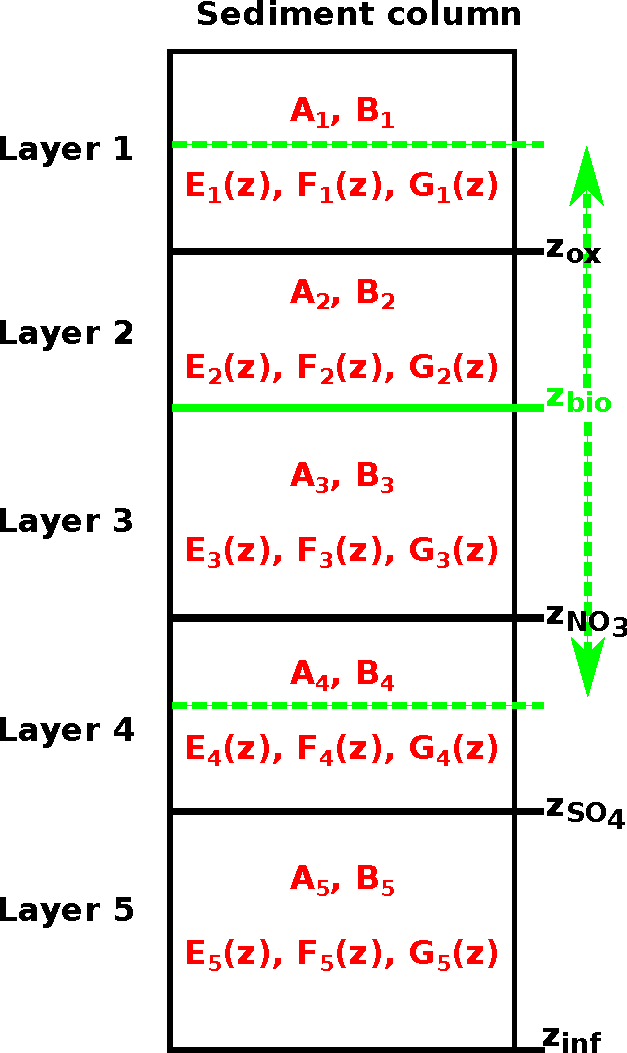
\includegraphics[width=0.3\textwidth]{figures/Boundary_Matching_zbio.pdf}
	\caption{Schematic of the generic boundary condition matching (GBCM) problem. Showing the resulting integration constants ($A_i,\ B_i$) and ODE solutions ($E_i,\ F_i,\ G_i$) for the different sediment layers and the variable 
	bioturbation boundary.}
	\label{fig:Boundary_matching_algo}
	\end{center}
\end{figure}
%\subsubsection*{Application in the model}\label{subsubsec:GBCM-Appl}

\subsubsection*{Solving the sediment layer stack}
Equations (\ref{Solution_matchsoln}), (\ref{Solution_Upper_transformed_basis_fct}) and (\ref{Solution_NEW_EFG}) can now be applied for each layer boundary, working up from the bottom of the sediments. 
The net result is to construct a piecewise solution with just two integration constants (coming from the lowest layer), which can then be solved for by applying one boundary condition for the sediment-water interface 
and one for the bottom of the sediments (e.g. a concentration condition at the bottom of the sediments, and a flux condition at the SWI).
% The key point here is that this is now an algorithm (rather than a fully-worked-out algebraic solution), which only ever has to solve a two-simultaneous-equation problem as above.

%\textbf{\textcolor{red}{TODO: Add figure, illustrating this e.g. for nitrate...}}

\subsubsection*{Abstracting out the bioturbation boundary}
The bioturbation boundary affects the diffusion coefficient of the modelled solutes and the conservation equation of organic matter which is available for mineralization. 
The boundary is particularly inconvenient as it can in principle occur in the middle of any ``geochemical'' layer and therefore generates multiple cases (compare Fig. \ref{fig:Boundary_matching_algo}). 
To simplify this for solutes, the ``piecewise solution construction'' above is used to abstract out the bioturbation boundary. 
An initial test for each layer is made to identify its ``bioturbation-status'' (fully bioturbated, fully non-bioturbated or crossing the bioturbation boundary) and (if needed) a piecewise solution is 
constructed by matching boundary conditions across the bioturbation boundary. 
The ``outside'' code therefore never needs to know whether it is dealing with a piecewise solution (i.e. matched across a bioturbation boundary) or a ``simple'' solution (i.e. the layer is fully bioturbated
or fully non-bioturbated).\\[1em]
In the code, this is performed by \textsf{\textbf{zTOC.prepfg\_l12}} which hands back a structure \textsf{ls} containing the ``bioturbation-status'' for each layer and (if needed) 
the description of the piecewise solution (coeffcients $c_1, c_2, c_3, c_4, d_1, d_2$ as above). So e.g. for sulfate, \textsf{\textbf{zTOC.prepfg\_l12}} is called three times at the beginning of \textsf{\textbf{zSO4.calcbc}} 
(one for each ``geochemical'' layer: oxic, suboxic, sulfidic) handing back three structures \textsf{ls} describing the layer's ``bioturbation-status'', abstracting away the bioturbation boundary and all associated conditional logic. 
When calculating the solutions for the different layers, the pre-calculated structure \textsf{ls} is passed to the function \textsf{\textbf{zTOC.calcfg\_l12}} which sorts out the correct
solution type to use.

\subsubsection{Coupling to an Earth System Model}\label{subsubsec:ESM_coupling}
% Describe what needs to be done/checked. Compare/use as example what I did with GENIE coupling. What are the if-clauses used? Input to OMEN-SED, output of OMEN-SED. 
\begin{figure}[tbp]
\begin{center}
	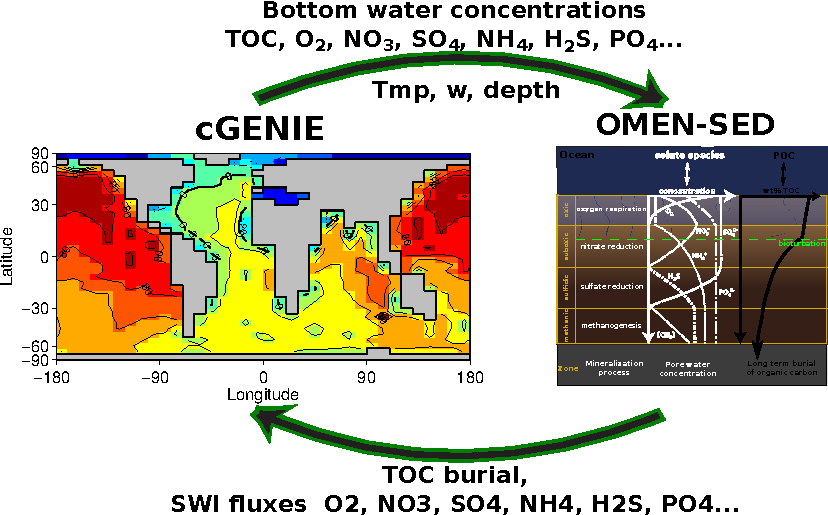
\includegraphics[width=0.8\textwidth]{figures/OMEN-GENIE-coupling.pdf}
	\caption{Schematic of the relationship between OMEN-SED (1.0) and GENIE. Arrows and accompanied text represent the information transferred between models. }
	\label{fig:OMEN-GENIE-coupling}
	\end{center}
\end{figure}

Here the coupling of OMEN-SED (1.0) to the GENIE Earth System model is described, in particular its incorporation into the sediment geochemistry model \citep[SEDGEM,][]{ridgwell_regulation_2007}. 
Results from pre-industrial experiments are presented in section \ref{subsec:GENIE-pre-ind}. Instead of remineralising POC completely at the seafloor, OMEN-SED (1.0) is called by SEDGEM for each grid point, 
passing over the bottom water concentrations of solutes ($\frac{mol}{kg}$, which is converted to $\frac{mol}{cm^3}$) and the flux of POC (\chem{POC_{flux}}, $\frac{cm^3}{cm^2\,yr}$, see Fig. \ref{fig:OMEN-GENIE-coupling}). 
\chem{POC_{flux}} is converted to $\frac{mol}{cm^2\,yr}$ assuming the average density of POC as 1.0 cm$^{3}$ g$^{-1}$. 
Other parameters passed over from GENIE are seafloor depth, local temperature and the partitioning of bulk POC into the slower and faster degrading pool 
(as GENIE represents a labile and a refractory POC fraction, see \citet{ridgwell_marine_2007}). 
For bottom water oxygen concentrations below 5 $\mu$mol kg$^{-1}$ the bioturbation depth is changed from 10 to 0.01 cm to account for the reduced presence of organisms under anoxia.  
The advection/sediment accumulation rate is taken from GENIE, whereas a minimum values of $w=0.5\frac{cm}{kyrs}$ is imposed as OMEN-SED (1.0) tends to be unstable for lower values. 
If the POC depositional flux is zero, OMEN-SED (1.0) is not called and all SWI-fluxes of solutes and the fraction of POC preserved in the sediments (\chem{POC_{pres}}) are set to zero.
Otherwise, the bulk \chem{POC_{flux}} is seperated into the labile and refractory component and the routine to calculate the sedimentary POC profiles is called. Here, the two POC depositional fluxes are first converted into SWI concentrations (in $\frac{mol}{cm^3}$) by solving Eq. (\ref{Eq_flux_divergence}) for z=0.
\textcolor{red}{TODO: From here:} Write about coupling and stoichiometries need to match with the ocean biogeochemical model. Also describe different options for POC degradation rates (i.e. globally invariant value, 
related to sedimentation rate or POC settling flux).

% For the solutes this is trivial; the OM flux is converted into a concentration (\chem{POC_{con}}, in $\frac{mol}{cm^3}$) using the sediment accumulation rate from GENIE ($w$, in $\frac{cm}{yr}$) as:
% \begin{equation}
%  \chem{POC_{con}} = \frac{1}{12}\cdot(1-\phi)\cdot \frac{\chem{POC_{flux}}}{w}
% \end{equation}
% where $\phi$ is the sediment porosity (-) and $\frac{1}{12}$ is the conversion of POC from $cm^3$ to $mol$ assuming the average density of POC as $1.0 \frac{cm^3}{g}$ .
OMEN-SED (1.0) then computes the resulting SWI-fluxes of solutes (in $\frac{mol}{cm^2\,yr^1}$) and the fraction of POC preserved in the sediments at a depth of 100 cm which are given back to GENIE. 
In order to reduce memory requirements the sediment profiles (e.g. as shown in Fig. \ref{fig:Sediment_profiles}) are by default not calculated by OMEN-SED (1.0), however, the information needed to do this once the experiment 
has terminated is passed over and saved in SEDGEM (i.e. the integration constants from the lowest layer $A_L,\ B_L$ and the ODE solutions $E_i,\ F_i,\ G_i$ for the different sediment layers $i$).
\textcolor{red}{TODO: check that is correct... e.g. need all ODE solutions but just IC from lowest layer? - why not calculated like this in matlab when calc. the profiles...?}



\section {Test Cases}

\subsection{Sediment profiles}\label{subsec:SedProfiles}
From Stolpovsky:
We selected sites where pore water data were available from key ocean settings including the continental
shelf (41 and 114 m), slope (241 and 1025 m), and deep sea (3073 m) (Figure 4). Two of these sites,
stations WE206 and 241 on the Washington and Mauritanian margin (respectively), are located in
high-nitrate-low-oxygen (HNLO) areas where oxygen-deficient waters impinge on the seafloor. 

Figure \ref{fig:Sediment_profiles} compares profiles calculated with OMEN-SED (1.0) to observations from different ocean depths taken at the Santa Barbara basin \citep[585 m, ][]{reimers_porewater_1996}, 
the Iberian margin (108 and 2213 m) and Naza\'e Canyon \citep[4298 m, ][]{epping_oxidation_2002}. 
Sediment-water interface characteristics and concentrations of total organic matter and all dissolved species in OMEN-SED (1.0) were set to the observed values where available (Table \ref{table:Profiles_BC}). 
The OM and pore water profiles were fitted by optimizing the OM partitioning into the fast and slow degrading pool and their respective first order degradation rate constants (priority given to reproduce the OM and \chem{O_2} profiles). 
For phosphorus the equilibrium concentration for authigenic P formation (\chem{PO_4^a}) was adjusted to fit the \chem{PO_4} concentration at $z_\infty$. 
For the two open Iberian margin stations (108 and 2213 m) OMEN-SED (1.0) fits all observations well. OMEN-SED (1.0) does especially well at depth 2213m by reproducing the deep \chem{O_2} penetration and the subsurface maximum in \chem{NO_3} 
concentration due to the nitrification of \chem{NH_4}. 
For the Santa Barbara basin (585 m) a misfit is observed for \chem{H_2S} and \chem{PO_4} in the upper 20 cm of the sediment. This can be explained by the presence of \chem{Mn^{2+}}, \chem{Fe^{2+}} and dissolved \chem{Fe} at this site which 
are either reduced to degrade OM and/or react with \chem{H_2S} to form iron sulfides, therefore inhibiting the rise in concentration of \chem{H_2S} \citep{reimers_porewater_1996}. 
Phosphorus is adsorbed to \chem{Fe} oxides and incorporated into carbonate fluorapatite (\chem{CFA}) which is not modelled explicitly in OMEN-SED (1.0).  \textcolor{red}{above correct/okay....?}
For the Naza\'e Canyon station (4298 m) satisfactory fits could be realised apart from \chem{NH_4}. However, also the original study \citep{epping_oxidation_2002} had the same problem using a more 
complex diagenetic model and suggested non-local solute exchange being responsible for the higher observed \chem{NH_4} concentrations.

\begin{sidewaysfigure}[tbp]
	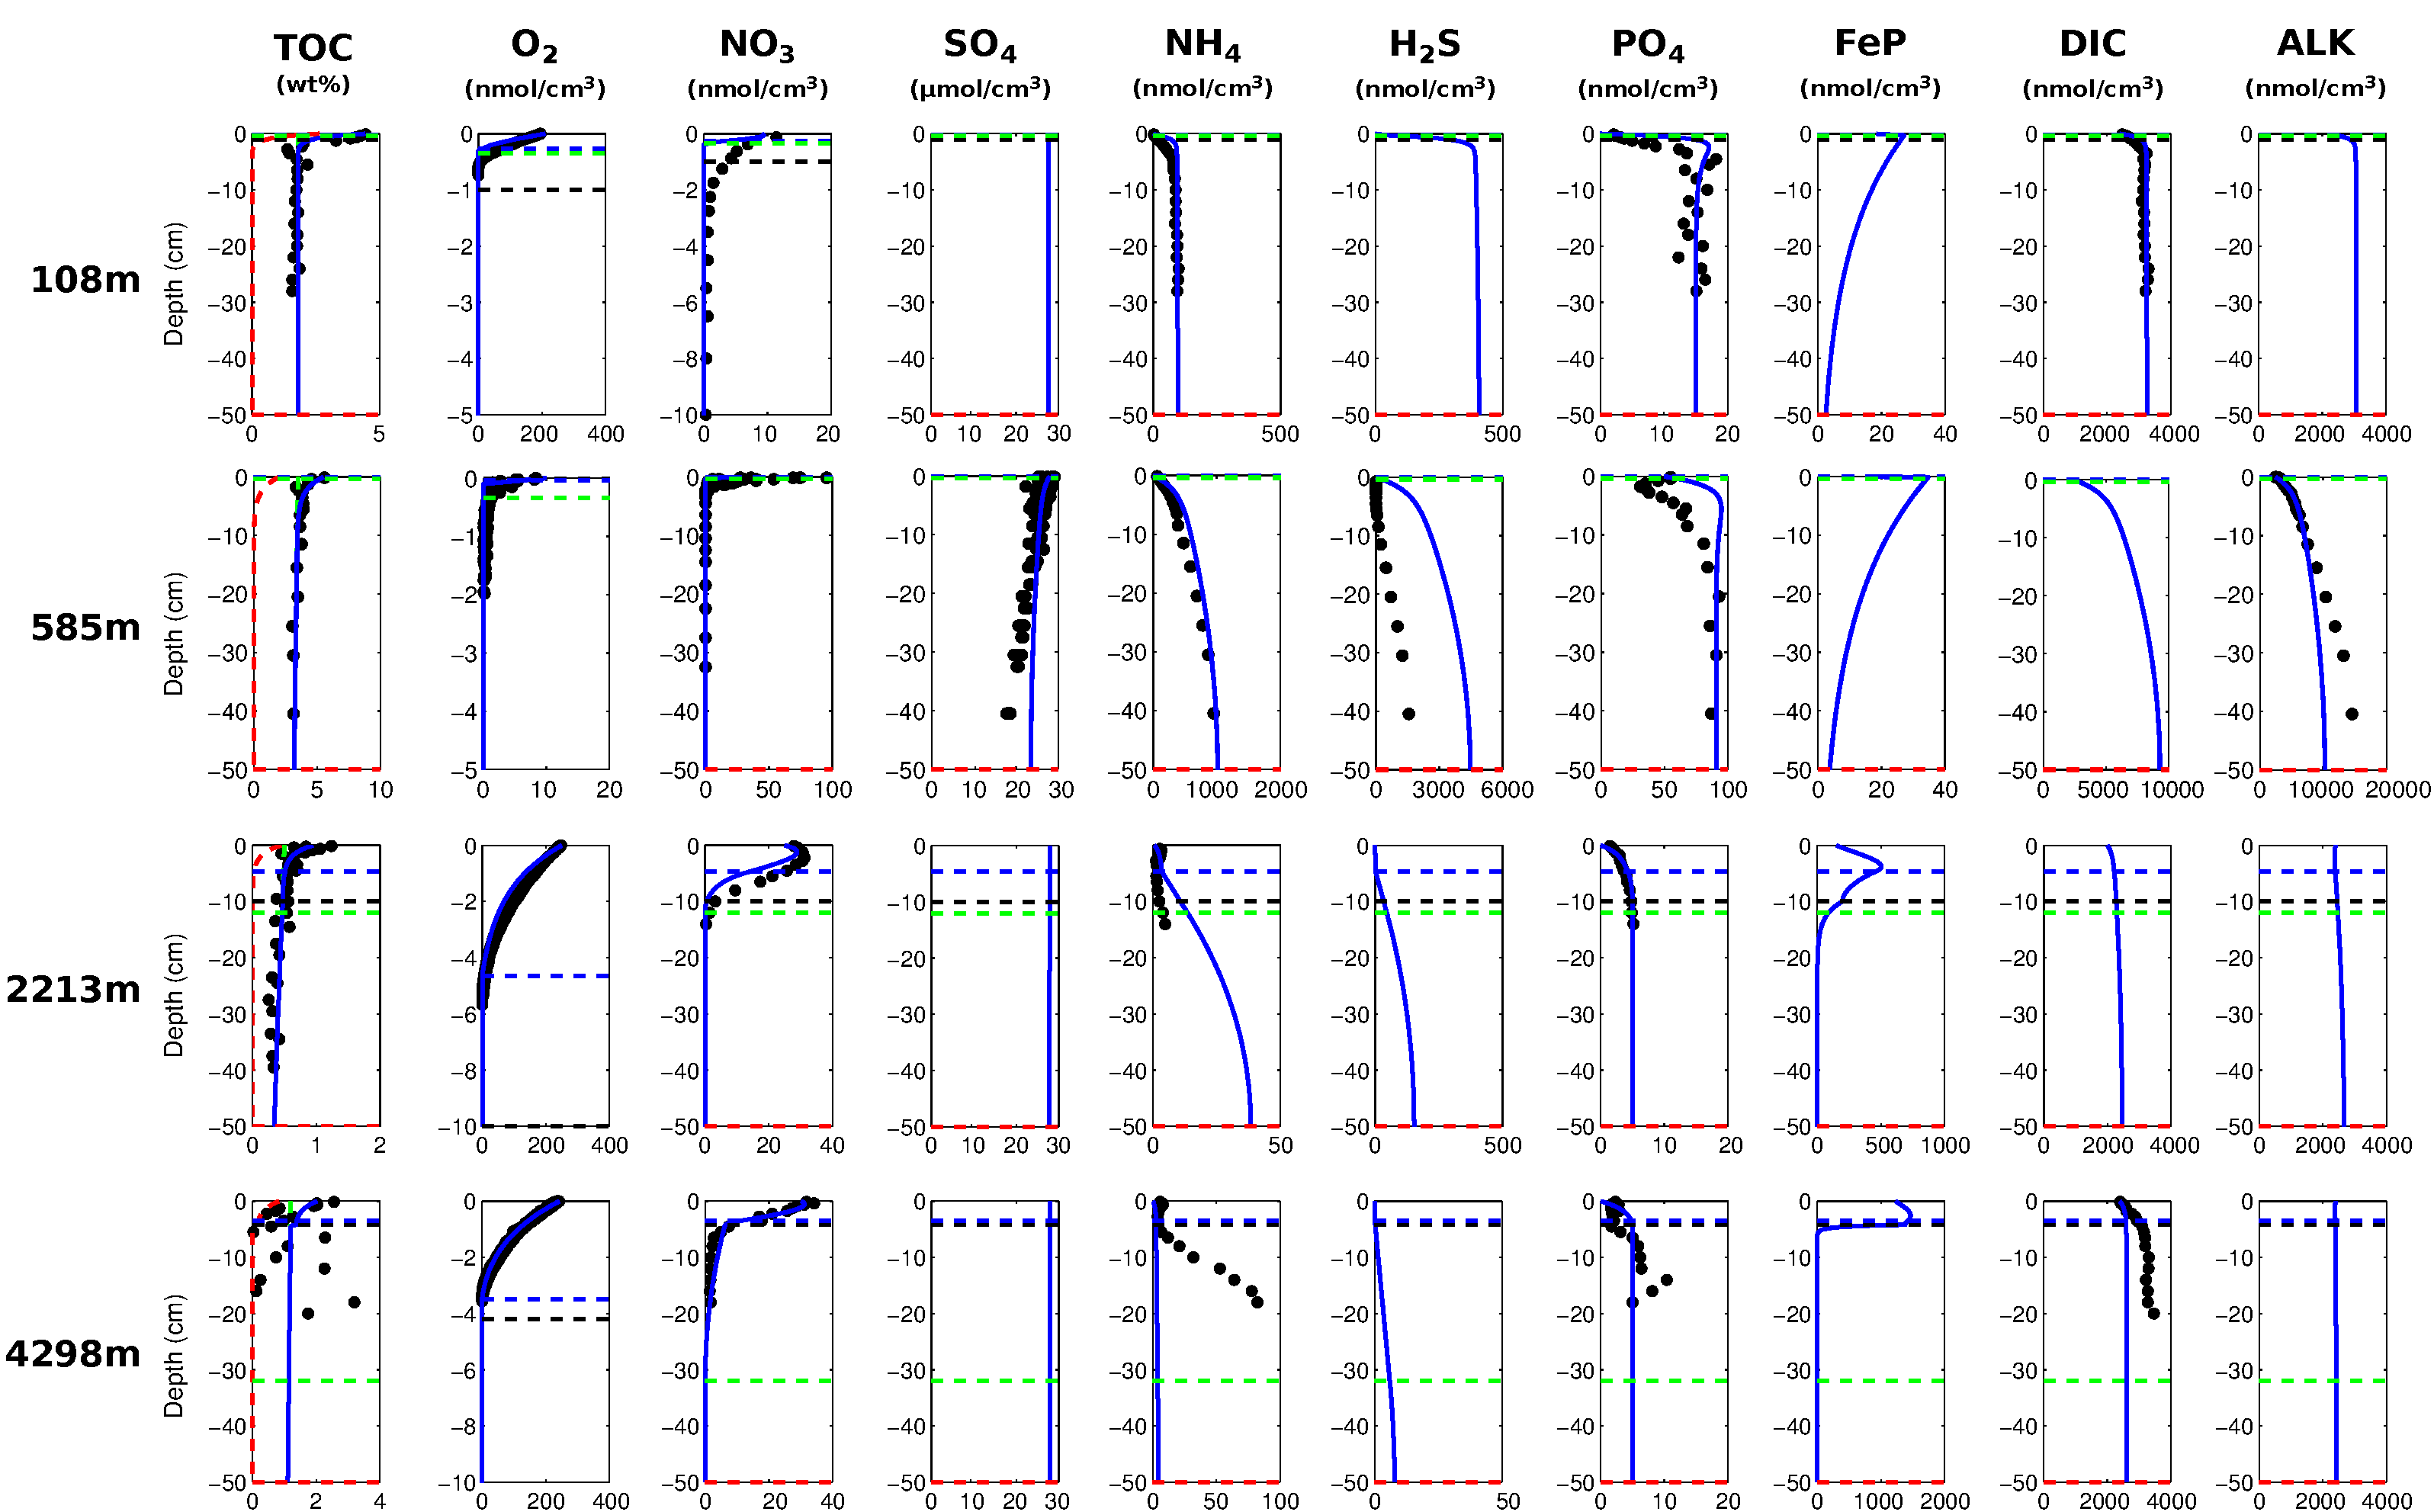
\includegraphics[width=1.0\textwidth]{figures/Profiles/0_ALL_PROFILES_COMBINED_1503.pdf}
	\caption{Modelled (curves) and measured (filled dots) dissolved and solid phase pore water profiles for four different sediment cores. Note that different 
	scales are used for different stations. The blue TOC curve represents the sum of the refractory (green) and labile (red) TOC fraction.}
	\label{fig:Sediment_profiles}
\end{sidewaysfigure}

\begin{table}[btp]
\caption{Model boundary conditions for the sampling stations in Figure \ref{fig:Sediment_profiles}. (For all sites DIC bottom water concentration of 
2,400 nanomole cm$^{-3}$ is assumed.)} 
% Note: Constant concentrations at all sites for \chem{SO_4} ($28000 \mu$mol cm$^{-3}$) and \chem{H_2S} (0.0 $\mu$mol cm$^{-3}$).}
\centering
% used for centering table
\begin{tabular}{l c c c c c c c c} 
% centered columns (15 columns)
\hline\hline
\multicolumn{8}{l}{\textbf{Sediment characteristics:}}\\
Depth & Temp. & $z_{\mathrm{bio}}$ & $D_{\mathrm{bio}}$  & \chem{TOC_1} & \chem{TOC_2} & \chem{k_1} & \chem{k_2}\\
 (m) & ($^{\circ}C$) & (cm) & (cm$^2$yr$^{-1}$) &(wt\%) & (wt\%) & (yr$^{-1}$) & (yr$^{-1}$)\\
\hline
108 & 12.5 & 1.0 & 0.02 & 2.64 & 1.8 & 0.65 & $1.0e^{-5}$ \\
585 & 5.85 & 0.01 & 0.02 & 2.0 & 3.5 & 0.2 & $8.0e^{-4}$\\
2213 & 3.2 & 10.0 & 0.17 & 0.45 & 0.5 & 0.1 & $4.0e^{-4}$\\
4298 & 2.5 & 4.2 & 0.18 & 0.83 & 1.2 & 0.052 & $1e^{-5}$\\
\hline\hline
\multicolumn{8}{l}{\textbf{Bottom water concentrations of solutes} (all in nanomole cm$^{-3}$):}\\
Depth & \chem{O_2} & \chem{NO_3} & \chem{SO_4} & \chem{NH_4} & \chem{H_2S} & \chem{PO_4} & \chem{PO_4^a} & \chem{Alkalinity}\\
%(m) & ($\frac{\mu mol}{cm^3}$) &  ($\frac{\mu mol}{cm^3}$) &  ($\frac{\mu mol}{cm^3}$) &  ($\frac{\mu mol}{cm^3}$) &  ($\frac{\mu mol}{cm^3}$)  &   ($\frac{\mu mol}{cm^3}$) &   ($\frac{\mu mol}{cm^3}$) \\
\hline
108 & 210 & 9.6 & 28,000 & 0.4 & 0.0 & 0.0 & 15.0 & 2,400\\
585 & 10 & 25.0 & 28,000 & 0.0 & 0.0 & 50.0 & 90.0 & 2,480\\
2213 & 250 & 25.0 & 28,000 & 0.6 & 0.0 & 0.0 & 5.0 & 2,400\\
4298 & 243 & 30.1 & 28,000 & 0.22 & 0.0 & 0.0 & 5.0 & 2,400\\
% inserts double horizontal lines
\end{tabular}
\label{table:Profiles_BC}
\end{table}


\subsection{Sensitivity Analysis}
Model parameters implicitly account for processes not explicitly described, they are notoriously difficult to constrain and a source of uncertainty for a numerical model. Sensitivity Analysis (SA) is a term used for mathematical 
techniques to investigate how the variations in the outputs ($y_1,\ ...,\ y_N$) of a numerical model can be attributed to variations in the different input parameters ($x_1,\ ...,\ x_M$) \citep{pianosi_sensitivity_2016}. 
Different types of sensitivity indices, which quantify this relative influence with a scalar $S_i$, can be calculated, ranging from simple one-at-a-time methods to statistical evaluations of the 
output distribution \citep[e.g. variance-based or density-based approaches][]{pianosi_sensitivity_2016}. Especially the latter indices are easy to interpret and to compare across different parameters and/or different model outputs as 
they generally take values between zero and one ($S_i \in [0, 1]$). An index of zero indicates a non-influential parameter and a higher value a more influential parameter. 
Here, we use SA mainly to identify which parameters have the largest impact on the different model outputs and therefore require careful calibration. 
% and if there is any factor whose variability has a negligible effects on specific outputs?
%Due to OMEN-SED's computational efficiency we are able to apply one of the approaches requiring higher numbers of model evaluations to compute the sensitivity index.  
As the probability density functions of our model outputs (i.e. the resulting SWI-fluxes) are generally highly-skewed towards extreme organic matter degradation rates (not shown) variance-based sensitivity indices are not very 
reliable uncertainty indicators \citep{pianosi_sensitivity_2016}. Rather than just considering the variance we employ the novel density-based PAWN method by \citep{pianosi_simple_2015} which considers the entire conditional and unconditional 
Cumulative Destribution Function (CDF) of the model output. % Probability Density Function (PDF) 
The sensitivity index of parameter $i$ is calculated as the difference between the two CDFs, i.e.
\begin{equation}
 S_i = \max_{x_i} \max_{y} | F_y(y) - F_{y|x_i}(y) |
\end{equation}
where $F_y(y)$ is the unconditional CDF of the output $y$ and $F_{y|x_i}(y)$ is the conditional CDF when the $i$-th parameter is fixed to $x_i$. For a more detailed description of the method we refer the interested reader to \citet{pianosi_simple_2015}. 
Due to the model complexity it is impossible to compute the sensitivity indices analytically therefore they are approximated from a Latin-Hypercube sampling of parameter inputs and calculated outputs.
We use PAWN as implemented within the Sensitivity Analysis for Everyone (SAFE) matlab toolbox \citep{pianosi_matlab_2015} to investigate 11 model parameters for ranges specified in Table \ref{table:SA_parameter_ranges}. 
We calculate sensitivity indices for all resulting SWI-fluxes from OMEN-SED for two idealised sediment conditions (see Table \ref{table:SA_2Cases}). 
The resulting indices (compare Fig. \ref{fig:SA_O2+NO3} for two examplary cases) are then translated into a color code and summarised in a pattern plot to simplify comparison (Fig. \ref{fig:Sensitivity_Analysis}). 
The most significant parameters for all model outputs are the degradation rate for the labile OM part ($\chem{k_1}$) and its share in the total OM pool ($\chem{f_1}$).
For the anoxic setup, where no oxidation occurs, the secondary redox parameters (i.e. $\gamma_\chem{NH_4},\ \gamma_\chem{H_2S}$) are essentially non-influential, however, they are getting more important for the oxic scenario. 
The $\chem{PO_4}$ SWI-flux appears to be insensitive under oxic conditions as the majority is absorbed to $\chem{Fe}$-oxides \textcolor{red}{correct....?}.


\begin{table}[btp]
\caption{Range of model parameters used for sensitivity analysis of model predicted output.} 
% Note: Constant concentrations at all sites for \chem{SO_4} ($28000 \mu$mol cm$^{-3}$) and \chem{H_2S} (0.0 $\mu$mol cm$^{-3}$).}
\centering
% used for centering table
\begin{tabular}{l l c c c c}
% centered columns (15 columns)
\hline\hline
Parameter & Description & Units & Minimum  & Maximum & Source\\
\hline
$\chem{k_1}$ & labile OM degradation constant & yr$^{-1}$ & $1e^{-4}$ & 5.0 & (1)\\
$\widetilde{\chem{k_2}}$ & order of refractory OM degradation & - & $1e^{-4}$ & $1e^{-1}$ &  (1)\\
 & constant ($k_2 = \widetilde{k_2} \cdot k_1$) & & &  &\\
$\chem{f_1}$ & fraction of labile OM & - & 0.02 & 0.98  & - \\
$K_{\chem{NH_4}}$ & Adsorption coefficient & - & 0.8 & 1.7  & (2) \\
$\gamma_\chem{NH_4}$ & $NH_4$ fraction oxidised &  & 0.5 & 1.0 & - \\
$\gamma_\chem{H_2S}$ &  $H_2S$ fraction oxidised  &  & 0.5 & 1.0 & - \\
$K_\chem{PO_4}^I$ & Adsorption coeff. oxic & - & 100.0 & 400.0  & (3) \\
$K_\chem{PO_4}^{II}$ & Adsorption coeff. anoxic & - & 1.3 & 2.0 & (3) \\
$k_{s}$ & kinetic P sorption & yr$^{-1}$  & 0.1 & 100.0 & (4, 5)\\
$k_{m}$ & Fe-bound P release & yr$^{-1}$  & 0.015 & 0.02 & (4, 5)\\
$k_{a}$ & authigenic P formation & yr$^{-1}$  & 0.001 & 10.0 & (4, 6)\\
\hline
Sources: &\multicolumn{5}{l}{(1) \citet{arndt_quantifying_2013}; (2): \citet{cappellen_cycling_1996}; (3): \citet{krom_adsorption_1980}}\\
&\multicolumn{5}{l}{(4): \citet{gypens_simple_2008}; (5): \citet{caroline_p_slomp_key_1996}; (6): \citet{cappellen_mathematical_1988}}
\end{tabular}
\label{table:SA_parameter_ranges}
\end{table}

\begin{table}[btp]
\caption{\textcolor{red}{Maybe in Suppl.} Model boundary conditions for the two idealised sediment conditions used for the sensitivity analysis (Fig. \ref{fig:Sensitivity_Analysis} and \ref{fig:SA_Color_ScatterPlots}). 
All solute concentrations are in nanomole cm$^{-3}$.} 
% Note: Constant concentrations at all sites for \chem{SO_4} ($28000 \mu$mol cm$^{-3}$) and \chem{H_2S} (0.0 $\mu$mol cm$^{-3}$).}
\centering
% used for centering table
\begin{tabular}{c c c c c c c c}
% centered columns (15 columns)
\hline\hline
Depth (m) & Temp. ({}$^\circ$C)& OC (wt\%) & \chem{O_2} & \chem{NO_3} & \chem{SO_4} & \chem{PO_4} & $z_{\mathrm{bio}}$ (cm)\\
\hline
400 & 8.0 & 2.0 & 0.0 & 40.0 & 28,000 & 40.0 & 0.001 \\
4000 & 1.5 & 1.0 & 300.0 & 20.0 & 28,000 & 40.0 & 10.0 \\
\hline
\end{tabular}
\label{table:SA_2Cases}
\end{table}


\begin{figure}[htbp]
\begin{center}
	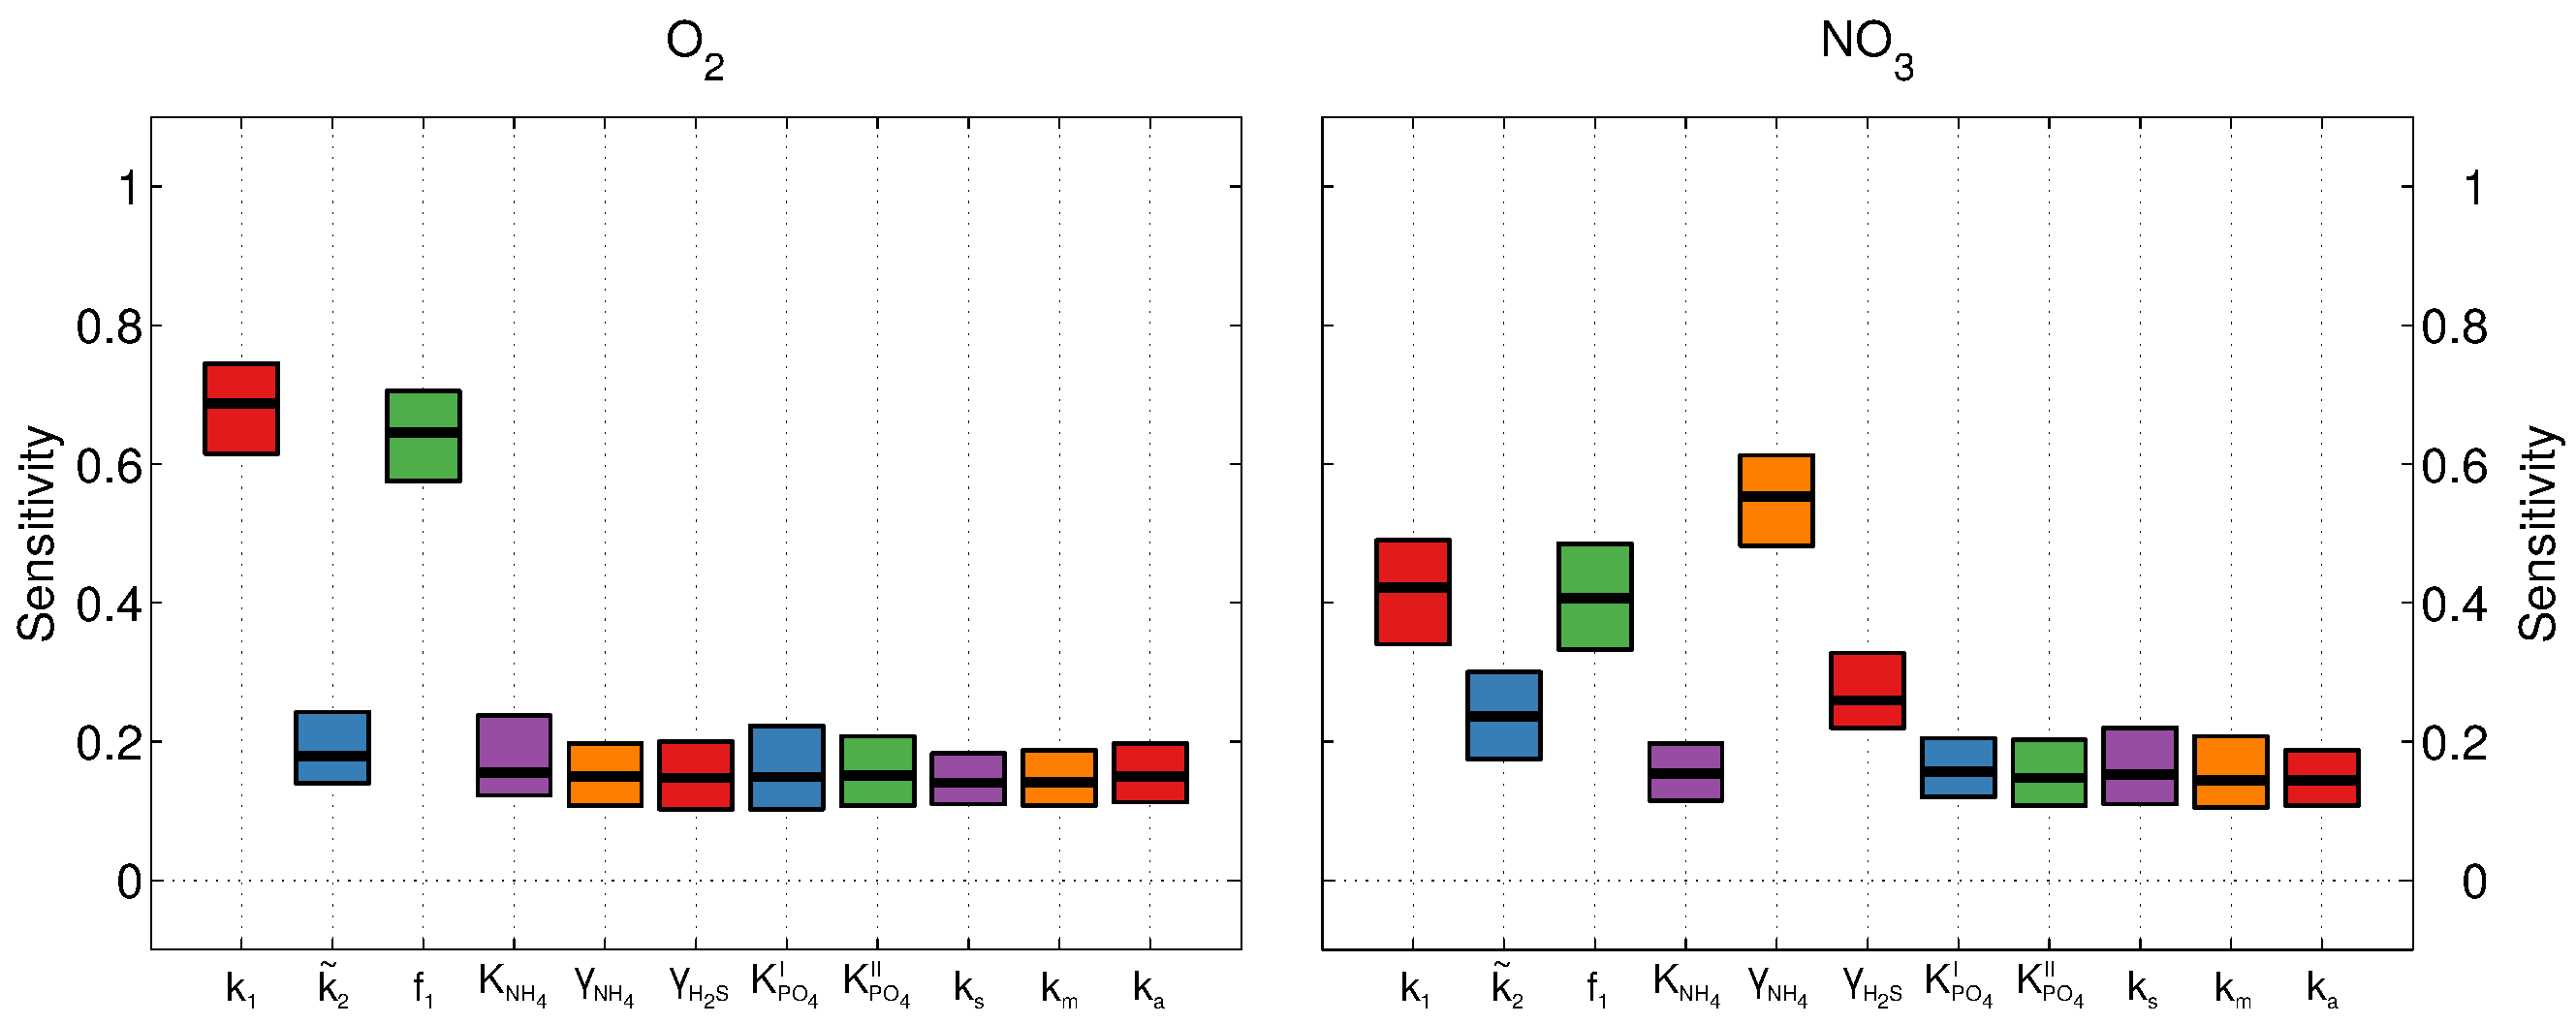
\includegraphics[width=1.0\textwidth]{figures/SA/SIndex_O_2+NO3_4000m.pdf}
	\caption{\textcolor{red}{Maybe in Suppl.} Box plot of parameter sensitivities for the $O_2$ and $NO_3$ SWI-flux for the 4000m oxic condition. 
	Average sensitivities (black lines) and 90\% condidence intervals using $N=11200$ model evaluations and $Nboot = 100$ bootstrap resamples.}
	\label{fig:SA_O2+NO3}
	\end{center}
\end{figure}


\begin{figure}[htbp]
\begin{center}
	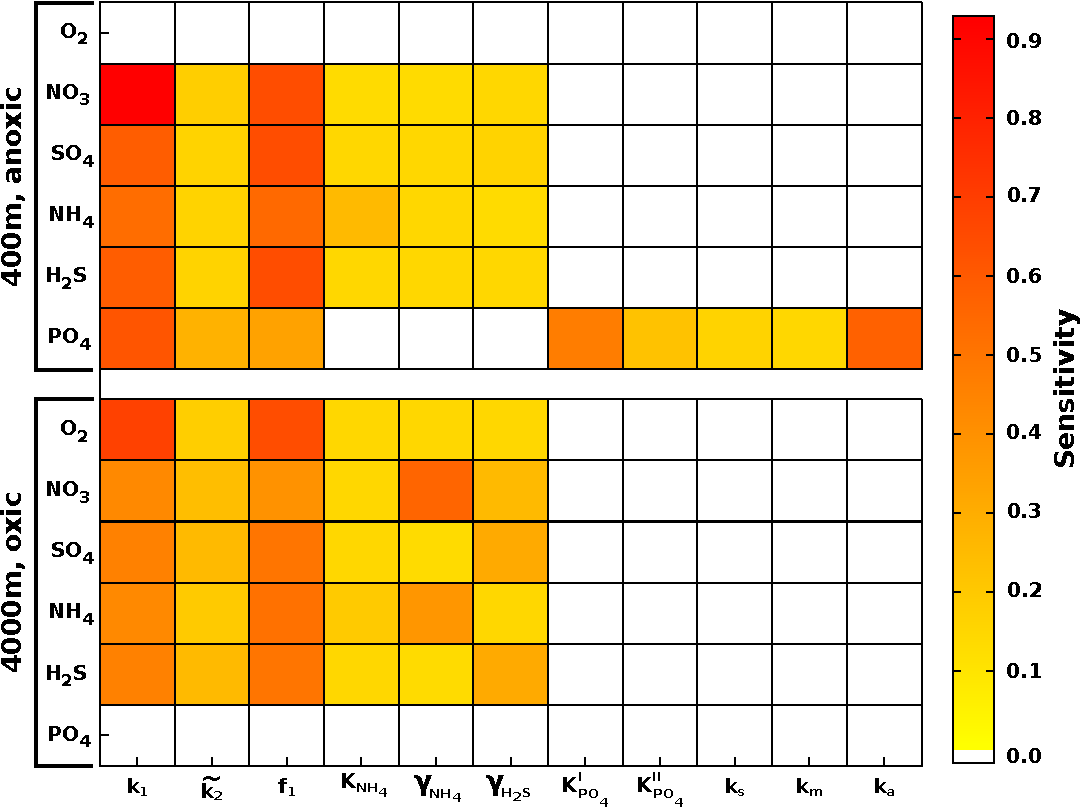
\includegraphics[width=1.0\textwidth]{figures/SA/0_KSIndex_ALL_OUTPUT_WHITE.pdf}
	\caption{Pattern plot, showing the output sensitivity for each SWI flux (i.e. the chemical compounds on the horizontal axis) and each input factor (i.e. the model parameters 
	on the vertical axis) for two idealised sediment cores. }
	\label{fig:Sensitivity_Analysis}
	\end{center}
\end{figure}

To test if OMEN-SED (1.0) is able to reproduce observed SWI-fluxes, the Latin-Hypercube sampling outputs are compared with a global database of benthic fluxes of $\chem{O_2}$ and $\chem{NO_3}$ \citep{bohlen_simple_2012}. 
The coloured scatter plots (Figure \ref{fig:SA_Color_ScatterPlots}) show that the observed fluxes fall well in the range of SWI-fluxes calculated with OMEN-SED (1.0). Also highlighted by the emergence of colour patterns 
in Figure \ref{fig:SA_Color_ScatterPlots} A+B are the strong interactions between the amount of labile OM  $\chem{f_1}$ and its degradation rate $\chem{k_1}$ for the resulting SWI-flux of the most powerful TEA available. 

% Conclude OM degradation rate highly important, reflects results from the literature ... important to calibrate... or run ensembles with different degradation rates which is easily possible with OMEN-SED. 
% Reality check, does OMEN-SED calculate realistic sediment-water interface fluxes!? Describe database of Stolpovsky and what we did. Add N to figures (i.e. data points from Stolpovsky).

\begin{figure}[htbp]
\begin{center}
	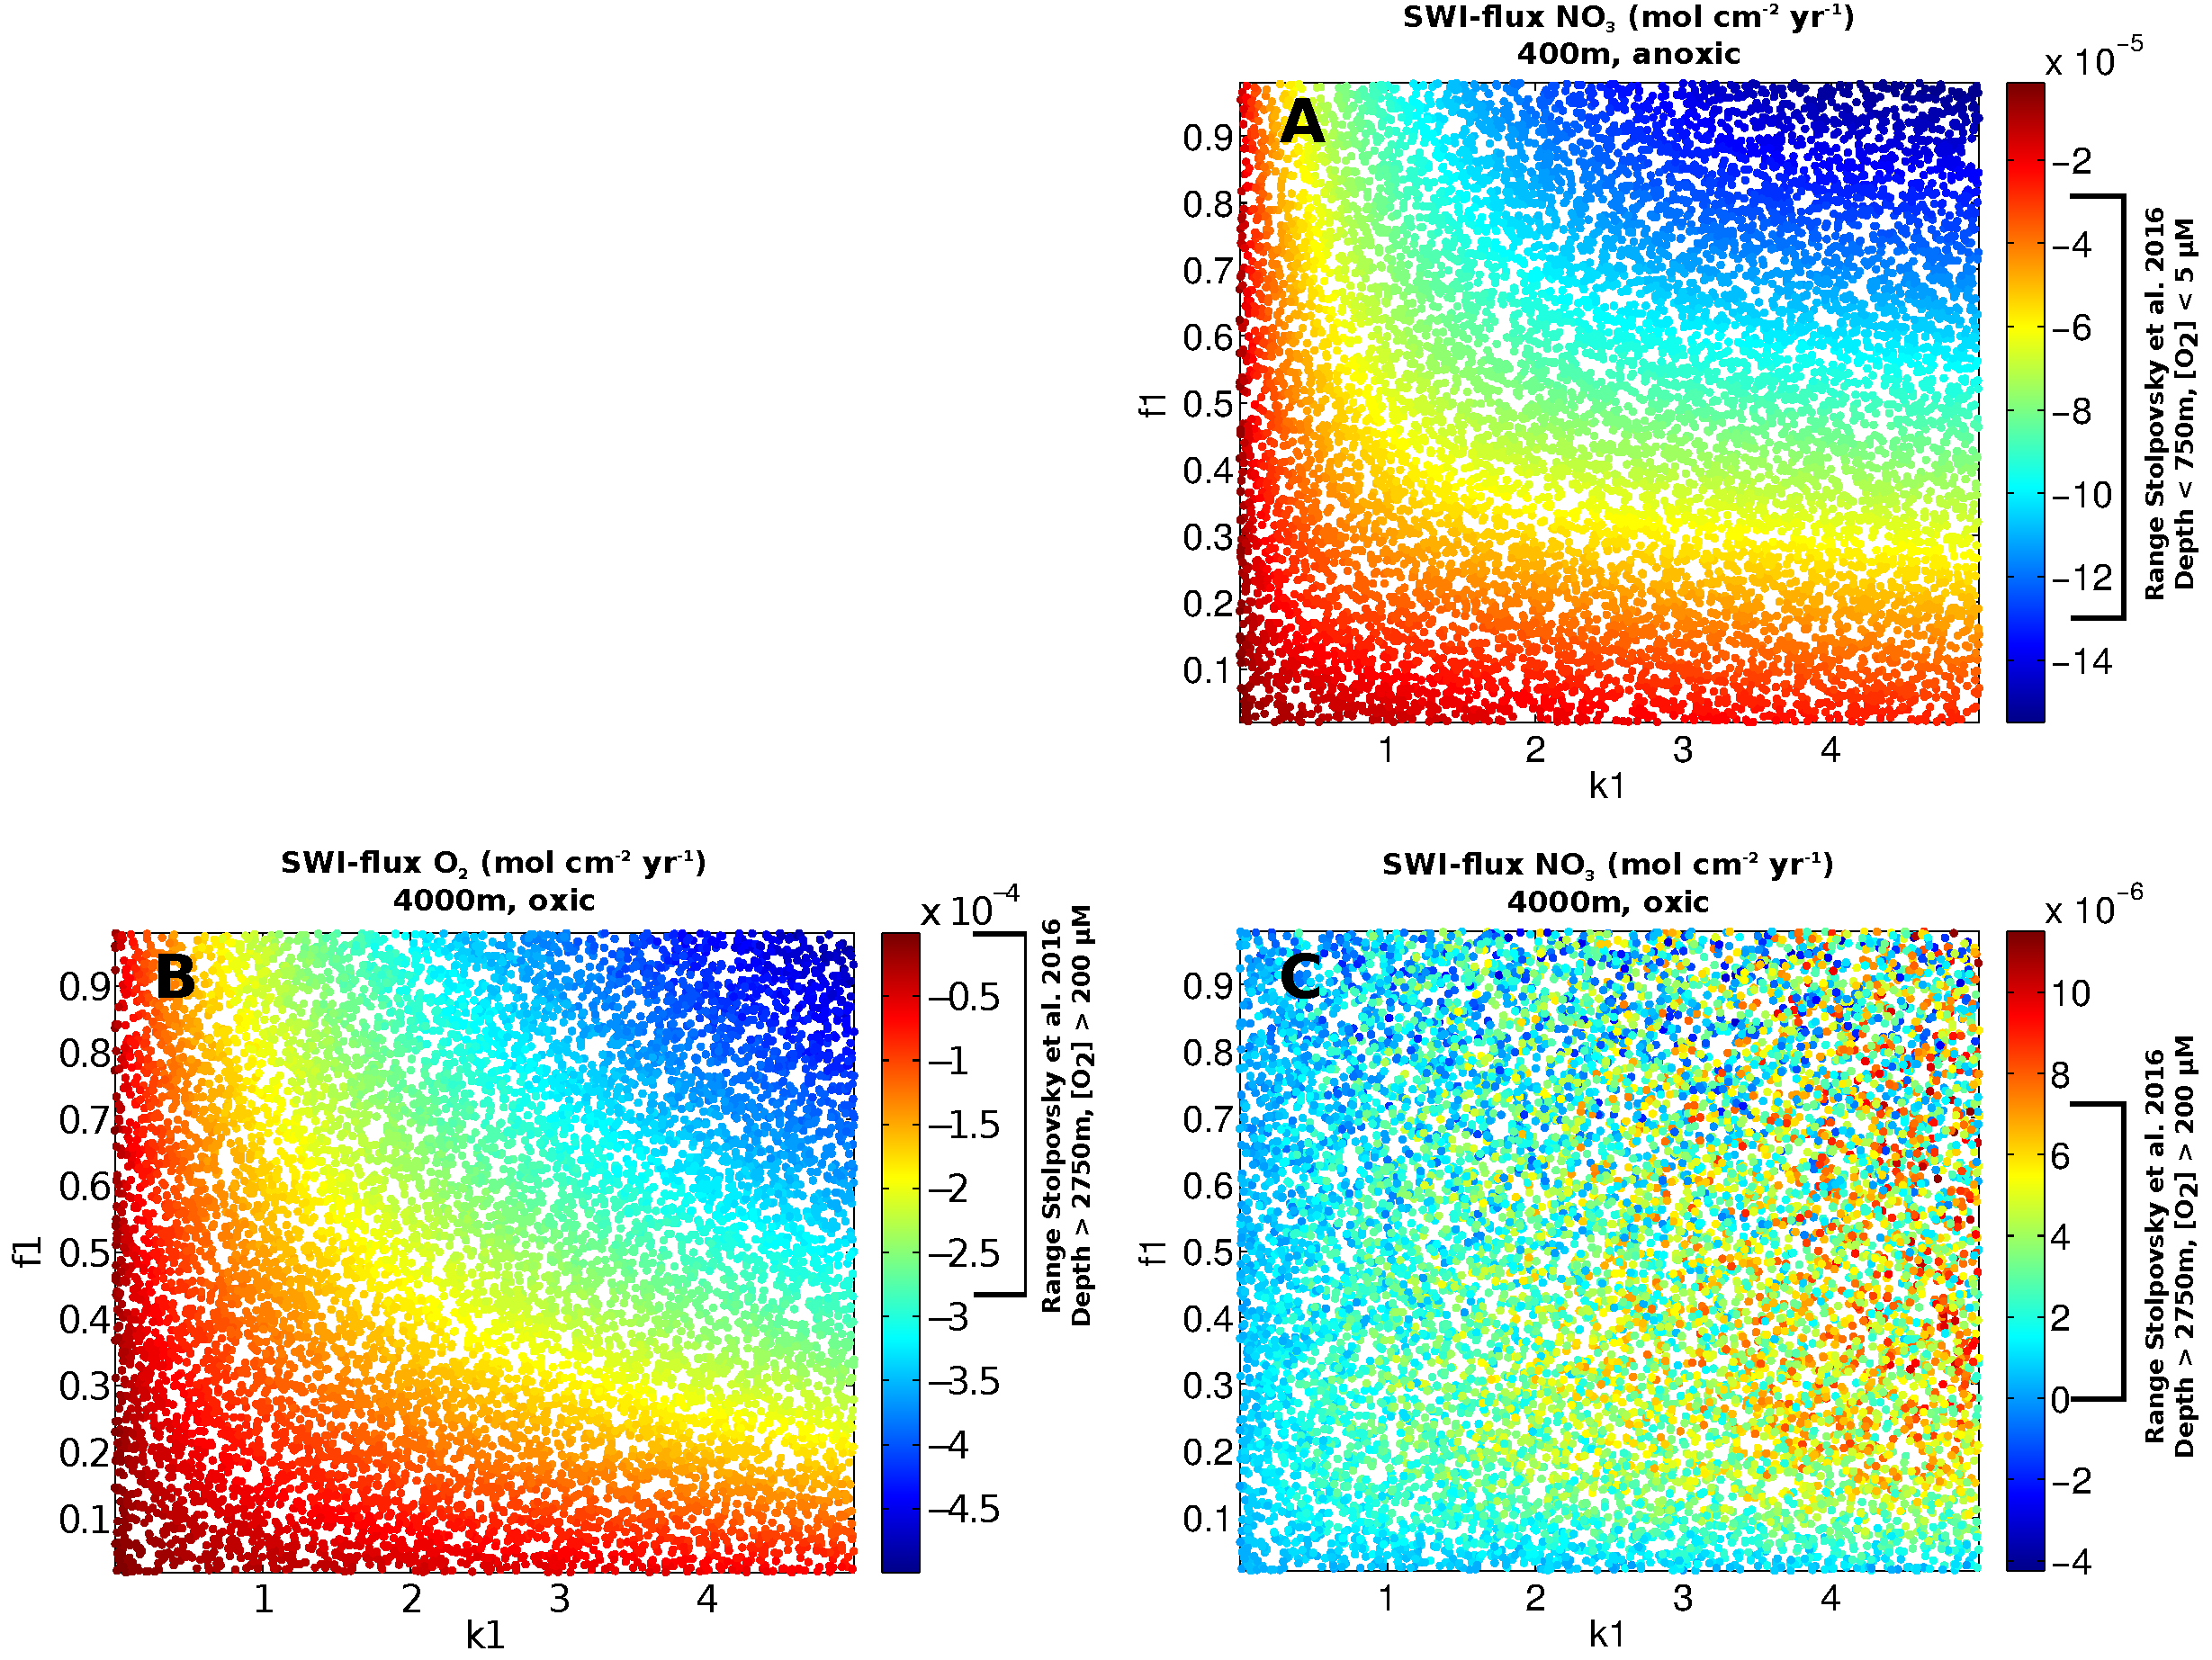
\includegraphics[width=1.0\textwidth]{figures/SA/k1_vs_f1_SWIflux_COMBINED.pdf}
	\caption{Coloured scatter plots ($\chem{k_1}$ vs $\chem{f_1}$) of resulting OMEN-SED (1.0) SWI-fluxes for the 400m anoxic (A: $\chem{NO_3}$) and 4000m oxic (B: $\chem{O_2}$, C: $\chem{NO_3}$) scenario. 
	Negative values representing flux from the water column into the sediments.
	Indicated area at the respective colour scale represents range of benthic fluxes in the global database of \citet{bohlen_simple_2012}. 
	\textcolor{red}{TODO: Add N and swap colour scale + add text: Low influx, High influx...}}
	\label{fig:SA_Color_ScatterPlots}
\end{center}
\end{figure}




\subsection{Benthic fluxes on a global scale}
Application to Seitert, 2004 OM, burwiczk see rate data and evaluation based on global data (Archer)

\subsection{GENIE pre-industrial}\label{subsec:GENIE-pre-ind}
From Boudreau book on POC fractions and their degradation constants:
Furthermore, it has been realized that there is not a single
organic matter type in sediments, but many. The data suggest that there is a reactive
fraction, k1, that decays within the top 10-20 cm of sediments, a more refractory
component, k2, that oxidizes on a scale of about ten to one hundred times longer, and a
third that is largely inert. The k2 material is largely, if not completely, subject to
anoxic decomposition. There is also a highly reactive component, say ko, that
decomposes on a seasonal time scale, largely at the sediment-water interface and in the
top centimeter of sediments, i.e. ko = 1-10 yr-1. Predictive correlations have, so far,
been applied only to k1 and k2.



From Stolpovsky: 
Our objective was to find an empirical function relating the depth distribution of POC mineralization to rain
rate (RRPOC). This is an attractive master variable because (i) POC fluxes to the seafloor are reasonably well
known and routinely computed by ESMs [e.g., Dunne et al., 2007] and (ii) POC reactivity appears to be
correlated with rain rate [Emerson et al., 1985; Murray and Kuivila, 1990; Soetaert et al., 1996; Boudreau, 1997;
Martin and Sayles, 2006].

Middelburg: Ocean margin sediments (<2000 m) account for about 85% of the material
accumulating in the ocean and about 80-90\% of the mineralization in marine sediments.  

\section{Scope of applicability and model limitations}


\conclusions  %% \conclusions[modified heading if necessary]
Not too bad this model...

\section {Code Availability}


\appendix
\section{Reaction Network}    %% Appendix A
\begin{sidewaystable}[tbp]
\caption{Primary pathways of organic matter degradation, secondary redox reactions and stoichiometries implemented in the reaction network.}
% title of Table
\centering
% used for centering table
\begin{tabular}{l l}
% centered columns (6 columns)
\hline\hline
%inserts double horizontal lines
 Pathway & Stoichiometry \\
\hline
& Primary Redox reactions\\
\hline
Aerobic degradation &  $ \chem{(CH_2O)_x(NH_3)_y(H_3PO_4)_z} + \mathrm{(x+2y)}\chem{O_2} + \mathrm{(y+2z)}\chem{HCO_3^-} \rightarrow \mathrm{(x+y+2z)}\chem{CO_2} + \chem{yNO_3^-} + \chem{zHPO_4^{2-}} + \mathrm{(x+2y+2z)}\chem{H_2O}$\\
Denitrification & $ \chem{(CH_2O)_x(NH_3)_y(H_3PO_4)_z} + \frac{\mathrm{(4x+3y)}}{5}\chem{NO_3^-} \rightarrow \frac{\mathrm{(2x+4y)}}{5}\chem{N_2} +  \frac{\mathrm{(x-3y+10z)}}{5}\chem{CO_2} + \frac{\mathrm{(4x+3y-10z)}}{5}\chem{HCO_3^-} 
		  + \chem{zHPO_4^{2-}} + \frac{\mathrm{(3x+6y+10z)}}{5}\chem{H_2O}$\\
Sulfate reduction &  $ \chem{(CH_2O)_x(NH_3)_y(H_3PO_4)_z} + \frac{\chem{x}}{2}\chem{SO_4^{2-}} + \mathrm{(y-2z)}\chem{CO_2} + \mathrm{(y-2z)}\chem{H_2O}\rightarrow \frac{\chem{x}}{2}\chem{H_2S} +  \mathrm{(x+y-2z)}\chem{HCO_3^-}  + \mathrm{y}\chem{NH_4^+} + \chem{zHPO_4^{2-}}$\\
Methanogenesis & $ \chem{(CH_2O)_x(NH_3)_y(H_3PO_4)_z} + \mathrm{(y-2z)}\chem{H_2O}\rightarrow \frac{\chem{x}}{2}\chem{CH_4} +  \frac{\mathrm{x-2y+4z}}{2}\chem{CO_2}  + \mathrm{(x-2z)}\chem{HCO_3^-} + \mathrm{y}\chem{NH_4^+} + \chem{zHPO_4^{2-}}$\\
\hline
& Secondary Redox reactions\\
\hline
Nitrification & $\chem{NH_4^++2O_2+2HCO_3^-}\rightarrow \chem{NO_3^-+2CO_2+3H_2O}$\\
Sulfide oxidation & $\chem{H_2S + 2O_2 + 2HCO_3^-} \rightarrow \chem{SO_4^{2-} + 2CO_2 + 2H_2O}$\\
AOM & $\chem{CH_4 + CO_2 + SO_4^{2-}} \rightarrow \chem{2HCO_3^- + H_2S}$\\
\hline
& Adsorption reactions and mineral precipitation\\
\hline
\chem{NH_4} adsorption & $\chem{NH_4^+} \xrightarrow{\mathrm{K_{NH_4}}} \chem{NH_4^+(ads)}$\\
\chem{P} ad-/desorption \textcolor{red}{???} & $\chem{PO_4^{2-}} \xrightarrow{\mathrm{K_{PO_4}^{I, II}}} \chem{PO_4^{2-}(ads)}; \qquad\quad \chem{HPO_4^{2-}} \xrightarrow{\mathrm{k_s}} \mathrm{Fe-bound\ P} \xrightarrow{\mathrm{k_m}} \chem{HPO_4^{2-}} $\\
\chem{CFA} precipitation & $\chem{PO_4^{2-}} \xrightarrow{\mathrm{k_a}} \chem{CFA}$ \\
\hline\hline
% inserts double horizontal lines
\end{tabular}
\label{table:Reaction_Network}
% is used to refer this table in the text
\end{sidewaystable}


\subsection{}                               %% Appendix A1, A2, etc.




\begin{acknowledgements}
Thank you...
\end{acknowledgements}


%% REFERENCES

%% The reference list is compiled as follows:

\newpage
\bibliographystyle{apalike} %Style of Bibliography: plain / apalike / amsalpha / ...
%\bibliography{/home/alex/BRL/bib/literature/VORbib.bib} %You need a file 'literature.bib' for this.
\bibliography{Sediment_model}


%% Since the Copernicus LaTeX package includes the BibTeX style file copernicus.bst,
%% authors experienced with BibTeX only have to include the following two lines:
%%
%% \bibliographystyle{copernicus}
%% \bibliography{example.bib}
%%
%% URLs and DOIs can be entered in your BibTeX file as:
%%
%% URL = {http://www.xyz.org/~jones/idx_g.htm}
%% DOI = {10.5194/xyz}


%% LITERATURE CITATIONS
%%
%% command                        & example result
%% \citet{jones90}|               & Jones et al. (1990)
%% \citep{jones90}|               & (Jones et al., 1990)
%% \citep{jones90,jones93}|       & (Jones et al., 1990, 1993)
%% \citep[p.~32]{jones90}|        & (Jones et al., 1990, p.~32)
%% \citep[e.g.,][]{jones90}|      & (e.g., Jones et al., 1990)
%% \citep[e.g.,][p.~32]{jones90}| & (e.g., Jones et al., 1990, p.~32)
%% \citeauthor{jones90}|          & Jones et al.
%% \citeyear{jones90}|            & 1990



%% FIGURES

%% ONE-COLUMN FIGURES

%%f
%\begin{figure}[t]
%\includegraphics[width=8.3cm]{FILE NAME}
%\caption{TEXT}
%\end{figure}
%
%%% TWO-COLUMN FIGURES
%
%%f
%\begin{figure*}[t]
%\includegraphics[width=12cm]{FILE NAME}
%\caption{TEXT}
%\end{figure*}
%
%
%%% TABLES
%%%
%%% The different columns must be seperated with a & command and should
%%% end with \\ to identify the column brake.
%
%%% ONE-COLUMN TABLE
%
%%t
%\begin{table}[t]
%\caption{TEXT}
%\begin{tabular}{column = lcr}
%\tophline
%
%\middlehline
%
%\bottomhline
%\end{tabular}
%\belowtable{} % Table Footnotes
%\end{table}
%
%%% TWO-COLUMN TABLE
%
%%t
%\begin{table*}[t]
%\caption{TEXT}
%\begin{tabular}{column = lcr}
%\tophline
%
%\middlehline
%
%\bottomhline
%\end{tabular}
%\belowtable{} % Table Footnotes
%\end{table*}
%
%
%%% NUMBERING OF FIGURES AND TABLES
%%%
%%% If figures and tables must be numbered 1a, 1b, etc. the following command
%%% should be inserted before the begin{} command.
%
%\addtocounter{figure}{-1}\renewcommand{\thefigure}{\arabic{figure}a}
%
%
%%% MATHEMATICAL EXPRESSIONS
%
%%% All papers typeset by Copernicus Publications follow the math typesetting regulations
%%% given by the IUPAC Green Book (IUPAC: Quantities, Units and Symbols in Physical Chemistry,
%%% 2nd Edn., Blackwell Science, available at: http://old.iupac.org/publications/books/gbook/green_book_2ed.pdf, 1993).
%%%
%%% Physical quantities/variables are typeset in italic font (t for time, T for Temperature)
%%% Indices which are not defined are typeset in italic font (x, y, z, a, b, c)
%%% Items/objects which are defined are typeset in roman font (Car A, Car B)
%%% Descriptions/specifications which are defined by itself are typeset in roman font (abs, rel, ref, tot, net, ice)
%%% Abbreviations from 2 letters are typeset in roman font (RH, LAI)
%%% Vectors are identified in bold italic font using \vec{x}
%%% Matrices are identified in bold roman font
%%% Multiplication signs are typeset using the LaTeX commands \times (for vector products, grids, and exponential notations) or \cdot
%%% The character * should not be applied as mutliplication sign
%
%
%%% EQUATIONS
%
%%% Single-row equation
%
%\begin{equation}
%
%\end{equation}
%
%%% Multiline equation
%
%\begin{align}
%& 3 + 5 = 8\\
%& 3 + 5 = 8\\
%& 3 + 5 = 8
%\end{align}
%
%
%%% MATRICES
%
%\begin{matrix}
%x & y & z\\
%x & y & z\\
%x & y & z\\
%\end{matrix}
%
%
%%% ALGORITHM
%
%\begin{algorithm}
%\caption{�}
%\label{a1}
%\begin{algorithmic}
%�
%\end{algorithmic}
%\end{algorithm}
%
%
%%% CHEMICAL FORMULAS AND REACTIONS
%
%%% For formulas embedded in the text, please use \chem{}
%
%%% The reaction environment creates labels including the letter R, i.e. (R1), (R2), etc.
%
%\begin{reaction}
%%% \rightarrow should be used for normal (one-way) chemical reactions
%%% \rightleftharpoons should be used for equilibria
%%% \leftrightarrow should be used for resonance structures
%\end{reaction}
%
%
%%% PHYSICAL UNITS
%%%
%%% Please use \unit{} and apply the exponential notation


\end{document}